% !TeX spellcheck = pl_PL
\documentclass[11pt]{aghdpl}
% \documentclass[en,11pt]{aghdpl}  % praca w języku angielskim

% Lista wszystkich języków stanowiących języki pozycji bibliograficznych użytych w pracy.
% (Zgodnie z zasadami tworzenia bibliografii każda pozycja powinna zostać utworzona zgodnie z zasadami języka, w którym dana publikacja została napisana.)
\usepackage[english,polish]{babel}

% Użyj polskiego łamania wyrazów (zamiast domyślnego angielskiego).
\usepackage{polski}

\usepackage[utf8]{inputenc}

% dodatkowe pakiety

\usepackage{mathtools}
\usepackage{amsfonts}
\usepackage{amsmath}
\usepackage{amsthm}

% --- < bibliografia > ---

\usepackage[
style=numeric,
sorting=none,
%
% Zastosuj styl wpisu bibliograficznego właściwy językowi publikacji.
language=autobib,
autolang=other,
% Zapisuj datę dostępu do strony WWW w formacie RRRR-MM-DD.
urldate=iso8601,
% Nie dodawaj numerów stron, na których występuje cytowanie.
backref=false,
% Podawaj ISBN.
isbn=true,
% Nie podawaj URL-i, o ile nie jest to konieczne.
url=false,
%
% Ustawienia związane z polskimi normami dla bibliografii.
maxbibnames=3,
% Jeżeli używamy BibTeXa:
backend=bibtex
]{biblatex}

\usepackage{csquotes}
% Ponieważ `csquotes` nie posiada polskiego stylu, można skorzystać z mocno zbliżonego stylu chorwackiego.
\DeclareQuoteAlias{croatian}{polish}

\addbibresource{Bibliography.bib}

% Nie wyświetlaj wybranych pól.
%\AtEveryBibitem{\clearfield{note}}


% ------------------------
% --- < listingi > ---

% Użyj czcionki kroju Courier.
\usepackage{courier}

\usepackage{listings}
\lstloadlanguages{TeX}

\lstset{
	literate={ą}{{\k{a}}}1
           {ć}{{\'c}}1
           {ę}{{\k{e}}}1
           {ó}{{\'o}}1
           {ń}{{\'n}}1
           {ł}{{\l{}}}1
           {ś}{{\'s}}1
           {ź}{{\'z}}1
           {ż}{{\.z}}1
           {Ą}{{\k{A}}}1
           {Ć}{{\'C}}1
           {Ę}{{\k{E}}}1
           {Ó}{{\'O}}1
           {Ń}{{\'N}}1
           {Ł}{{\L{}}}1
           {Ś}{{\'S}}1
           {Ź}{{\'Z}}1
           {Ż}{{\.Z}}1,
	basicstyle=\footnotesize\ttfamily,
}

% ------------------------

\AtBeginDocument{
	\renewcommand{\tablename}{Tabela}
	\renewcommand{\figurename}{Rys.}
}

% ------------------------
% --- < tabele > ---

\usepackage{array}
\usepackage{tabularx}
\usepackage{multirow}
\usepackage{booktabs}
\usepackage{makecell}
\usepackage[flushleft]{threeparttable}

% defines the X column to use m (\parbox[c]) instead of p (`parbox[t]`)
\newcolumntype{C}[1]{>{\hsize=#1\hsize\centering\arraybackslash}X}


%---------------------------------------------------------------------------

\author{Grzegorz Nieużyła}
\shortauthor{G. Nieuźyła}

%\titlePL{Przygotowanie bardzo długiej i pasjonującej pracy dyplomowej w~systemie~\LaTeX}
%\titleEN{Preparation of a very long and fascinating bachelor or master thesis in \LaTeX}

\titlePL{Implementacja systemu uwierzytelniania z~zastosowaniem Negatywnych Baz Danych}
\titleEN{Implementation of authentication system using Negative Databases}


\shorttitlePL{Implementacja systemu uwierzytelniania z~zastosowaniem Negatywnych Baz Danych} % skrócona wersja tytułu jeśli jest bardzo długi
\shorttitleEN{Implementation of authentication system using Negative Database}

\thesistype{Praca dyplomowa inżynierska}
%\thesistype{Master of Science Thesis}

\supervisor{dr inż. Piotr Szwed}
%\supervisor{Marcin Szpyrka PhD, DSc}

\degreeprogramme{Informatyka}
%\degreeprogramme{Computer Science}

\date{2020}

\department{Katedra Informatyki Stosowanej}
%\department{Department of Applied Computer Science}

\faculty{Wydział Elektrotechniki, Automatyki,\protect\\[-1mm] Informatyki i Inżynierii Biomedycznej}
%\faculty{Faculty of Electrical Engineering, Automatics, Computer Science and Biomedical Engineering}

\acknowledgements{}


\setlength{\cftsecnumwidth}{10mm}

%---------------------------------------------------------------------------
\setcounter{secnumdepth}{4}
\brokenpenalty=10000\relax

\begin{document}

\titlepages

% Ponowne zdefiniowanie stylu `plain`, aby usunąć numer strony z pierwszej strony spisu treści i poszczególnych rozdziałów.
\fancypagestyle{plain}
{
	% Usuń nagłówek i stopkę
	\fancyhf{}
	% Usuń linie.
	\renewcommand{\headrulewidth}{0pt}
	\renewcommand{\footrulewidth}{0pt}
}

\setcounter{tocdepth}{2}
\tableofcontents
\clearpage

% !TeX spellcheck = pl_PL
\chapter{Wprowadzenie}
\section{Cele pracy}
Celem niniejszej pracy jest implementacja i~przetestowanie systemu uwierzytelniania oferującego większe bezpieczeństwo
niż standardowy schemat generowania skrótu hasła za pomocą funkcji generacji klucza (np. \textit{PBKDF2}, \textit{bcrypt})
i~przechowywaniu w~standardowej (pozytywnej) bazie danych.
    
Jak wynika z~raportu Google\cite{google-poll} większość internautów ma problem z~zachowaniem zasad bezpieczeństwa dotyczącego 
używania mediów społecznościowych i~portali internetowych. $66\%$ procent badanych przyznało się do używania jednego hasła do różnych kont. 
W~przypadku wykradzenia bazy danych pojedynczego portalu i~uzyskaniu postaci jawnych haseł istnieje ryzyko uzyskania dostępu również do innych aplikacji
przez atakującego.

Główną przyczyną nadużywania jednego hasła jest konieczność zapamiętania danych logowaniu do wielu stron internetowych -- $75\%$ internautów ma problem z~ich zarządzeniem.
  
Istnieje szereg metod, które indywidualny użytkownik może zastosować w~celu polepszenia swojego bezpieczeństwa w~Internecie, ale nie cieszą
się one dużą popularnością. Według raportu tylko $37\%$ internautów używa uwierzytelnienia wielopoziomowego, a~menadżerów haseł
umożliwiających stosowanie różnych i~silnych danych logowania -- tylko $15\%$.

Częściowym rozwiązaniem tego problemu może być wprowadzenie dodatkowych warstw bezpieczeństwa bezpośrednio w~systemach uwierzytelniania
w~celu utrudnienia uzyskania nieautoryzowanego dostępu do wrażliwych danych. Takie podejście pozwoli podnieść bezpieczeństwo wszystkich użytkowników,
niezależnie od indywidualnych preferencji i~nawyków.
 
Założeniem systemu jest zamienienie reprezentacji w~sposób jawny na Negatywną Bazę Danych ($NDB$) co pozwoli dodać 
dodatkową warstwę bezpieczeństwa która znacząco utrudni uzyskanie haseł użytkownika w~przypadku kradzieży bazy danych.

W~tym celu opisałem różne algorytmy prezentowane w~dostępnej literaturze, przedstawiłem schemat ich działania i~porównałem
je pod względem bezpieczeństwa. 

Rezultatem wyjściowym algorytmów generacji $NDB$ jest zbiór ciągów tekstowych, które można jednoznacznie sprowadzić 
do zbioru formuł logicznych CNF, dlatego przeprowadzone zostały testy z~wykorzystaniem solwerów SAT mające na celu 
zasymulowanie ataku na powstałą $NDB$.

Koncept negatywnej reprezentacji danych wywodzi się z immunologii. Badania wykazały, że limfocyty $T$~wykorzystują
podobny proces w celu rozróżnienia między sobą i~innymi komórkami \cite{T-cells}.

\section{Zawartość pracy}


















% !TeX spellcheck = pl_PL
\chapter{Negatywne Bazy Danych - opis teoretyczny}
\section{Opis działania}
Główną operacja wykonywalną na $NDB$ jest sprawdzenie czy dany rekord znajduje się w bazie. Przyjmując $U$ 
jako oznaczenie uniwersum języka binarnego o~długości $l$ a $DB$ jako zbiór wszystkich rekordów, każdy o~długości $l$,
$NDB$ przechowuje zbiór $U - DB$ \cite{NRI-Esponda}. Takie dane są niepraktycznie do zareprezentowania w postaci nieskompresowanej z~uwagi na wielkość, dlatego
stosuje się wyrazy nad alfabetem $\{0,1,*\}$ gdzie symbol $*$ może oznaczać zarówno $0$ lub $1$ w jawnej reprezentacji bitowej.
Pozycje na których znajduje się wartość $0$ lub $1$ są \textit{ustalone} a z~wartością $*$ - \textit{nieustalone}.

Każdy taki wyraz odpowiada jednemu lub wielu elementom $U - DB$ i~jest sprowadzany do formuły logicznej (Tabela \ref{Tbl:NDB-logform}).
Z założenia algorytm sprawdzający przynależność do $DB$ sprawdza czy jakakolwiek formuła z~$NDB$ jest spełniana przez dany rekord. 
Dane znajdują się w $DB$ wtedy i~tylko wtedy gdy żadna formuła nie zostanie spełniona. 

Taki model działania wymusza na danych stałą wielkość,
co jednak nie stanowi problemu w przypadku przechowywania skrótów haseł które mają stałą, zależną od konkretnego algorytmu długość.
Dla danych o~zmiennych rozmiarach (np. nazwy użytkownika) można zastosować funkcję hashującą lub algorytmy zwiększające długość ciągu bitowego do stałej wartości typu PKCS\#5 lub PKCS\#7.
Należy jednak pamiętać, że zwiększenie długości rekordu znacznie wydłuża czas generacji bazy oraz zajmowaną pamięć. 

\begin{table}[h]
    \caption{Reprezentacja formuł logicznych za pomocą NDB}
    \centering
    \label{Tbl:NDB-logform}
    \begin{tabular}{|l|l|}
        \hline
        rekord NDB & formuła logiczna                       \\ \hline
        011*       & $\neg{x_1} \land x_2 \land x_3$        \\ \hline
        0*01       & $\neg{x_1} \land \neg{x_3} \land x_4 $ \\ \hline
        111*       & $x_1 \land x_2 \land x3$               \\ \hline
    \end{tabular}
\end{table}

\section{Zastosowanie w systemach uwierzytelniania}
NDB może być wykorzystana w każdym systemie, gdzie podstawową operacją na danych jest sprawdzenie czy
dany rekord znajduje się w bazie. Jednym z~najpopularniejszych systemów uwierzytelniania jest metoda oparta na loginie i~haśle.
Użytkownik danej aplikacji przy zakładaniu konta podaje hasło, które następnie warstwa serwerowa danej aplikacji przechowuje jako wynik nieodwracalnej funkcji hashującej.

W przypadku nieautoryzowanego dostępu do bazy danych i~używanego algorytmu uzyskiwania skrótu z~hasła, atakujący może uzyskać 
wartość pierwotną mało skomplikowanych haseł za pomocą np. metody słownikowej. Modyfikując powyższy algorytm 
składując skróty jako rekordy w NDB uniemożliwiamy iterację wszystkich danych, jednocześnie pozostawiając
łatwy dostęp do informacji czy użytkownik o~podanym loginie i~haśle ma dostęp do aplikacji.

\section{Algorytmy generacji Negatywnych Baz Danych}
\subsection{Algorytm prefiksowy}
\label{sec:prefix-alg}
Najprostszym ze sposobów generowania Negatywnych Baz Danych jest zaproponowany przez Fernando Esponda 
algorytm prefiksowy \cite{NRI-Esponda, Esponda2004EnhancingPT}. Został on opracowany w celu udowodnienia
że proces generowania NDB z~rekordów $DB$ jest możliwy w~rozsądnej złożoności czasowej i~pamięciowej.
\\\\\\
\begin{algorithm}[H]
    \SetAlgoLined
    
    \KwData{$DB$ - zbiór rekordów do zareprezentowania w NDB, $l$ - liczba rekordów w $DB$}
    \KwResult{Zbiór rekordów NDB}
    $Prefix_n(V)$ - Prefiks n-znakowy rekordu $V$\\
    $len(V)$ - Długość rekordu $V$\\
    $W_i$ = \{\};\\
    i = 0;\\
    \While{i < l}{
        $W_{i+1}$ = Zbiór wszystkich $i+1$-znakowych ciągów bitowych $V_p$ nie będących prefiksem żadnego rekordu $DB$ i~dla których $Prefix_i(V_p) \in W_i$\\
        \ForEach{$V_p$ in $W_{i+1}$}{
            Stwórz rekord NDB o~długości $l$ którego $V_p$ jest prefiksem a na pozostałych pozycjach jest symbol $*$ i~dodaj do zbioru wyjściowego NDB
            
        }
        i = i + 1;\\
        $W_i$ = Zbiór wszystkich $i$-znakowych prefiksów rekordów $DB$
    }
    
    \caption{Algorytm prefiksowy}
    \label{alg:prefix}
\end{algorithm}
~\\\\


Powyższa metoda polega na generowaniu coraz dłuższych prefiksów które nie pokrywają się ze zbiorem $DB$.
W ten sposób na początku tworzone są rekordy odpowiadające znacznej części $U~-~DB$. Czasami występuje potrzeba zdefiniowania pewnych rekordów explicite bez wykorzystania symbolu $*$ jeżeli każdy możliwy prefiks jest także prefiksem rekordu z~$DB$. 
Przykładowy wynik działania znajduje się w tabeli \ref{tbl:prefix_results}.

\begin{table}[h]
    \centering
    \begin{tabular}{|l|l|l|}
        \hline
        DB   & U - DB & NDB  \\ \hline
        0000 & 0001   & 10** \\
        0110 & 0011   & 010* \\
        0010 & 0100   & 111* \\
        1101 & 0101   & 0001 \\
        & 0111   & 0011 \\
        & 1000   & 0111 \\
        & 1001   & 1100 \\
        & 1010   &      \\
        & 1011   &      \\
        & 1100   &      \\
        & 1110   &      \\
        & 1111   &      \\ \hline
    \end{tabular}
    \caption{Rezultat działania algorytmu prefiksowego}
    \label{tbl:prefix_results}
\end{table}



Algorytm prefiksowy jest deterministyczny i~każdy powstały rekord reprezentuje unikalną, nie pokrywającą się część $U~-~DB$ \cite{NRI-Esponda}.
Powoduje to, że algorytm uzyskiwania zbioru $DB$ z~otrzymanej $NDB$ nie wymaga sprowadzenia do problemu SAT. Wystarczy jedynie odpowiednio posortować rekordy i~wyznaczyć przedziały pomiędzy nimi.

Czas wykonywania procedury wynosi $O(l|DB|)$, jednak w~przypadku zapisywania wyniku do bazy wzrasta do $O(l^2|DB|)$ gdyż konieczna jest serializacja każdego rekordu.
Złożoność obliczeniowa dla optymalnej implementacji wynosi $O(l|DB|)$ w~przypadku gdy poprzednio generowane rekordy $NDB$ nie są przetrzymywane w~pamięci. 
Dla danego zbioru $DB$ generowane jest $O(l|DB|)$ rekordów co sprowadza się do wielkości powstałej bazy danych wynoszącej $O(l^2|DB|)$.
\subsection{Algorytm \textit{Randomize\_NDB}}
Algorytm prefiksowy generuje poprawne rekordy $NDB$, jednak nie jest praktyczny w~żadnych zastosowaniach związanych
z~bezpieczeństwem, ponieważ wynik jego działania jest stosunkowo prosto sprowadzić do postaci pozytywnej. 
Aby temu zaradzić, Fernando Esponda w~swojej pracy\cite{NRI-Esponda} zaproponował 
niedeterministyczny algorytm mający na celu wprowadzić rekordy które nie odpowiadają jedynie prefiksom elementów
z $U - DB$ i~są trudniejsze do odwrócenia.

\begin{algorithm}[H]
    \SetAlgoLined
    
    \KwData{$DB$ - zbiór rekordów do zareprezentowania w~NDB, $l$ - liczba rekordów w~$DB$}
    \KwResult{Zbiór rekordów NDB}
    $Prefix_n(V)$ - Prefiks n-znakowy rekordu $V$\\
    $len(V)$ - Długość rekordu $V$\\
    $\pi$ = losowa permutacja o~długości $|V_{pe}|$\\
    $W_i$ = zbiór wszystkich ciągów $l$-bitowych\\
    $\pi(DB)$ $\equiv$ $\{\pi(V) ~|~ V \in DB\}$\\
    $i$ = $\left \lceil{log_2(l)}\right \rceil$;\\
    \While{$i < l$ \textbf{and} $W_i \neq \emptyset $}{
        $W_{i+1}$ = Zbiór wszystkich $i+1$-znakowych ciągów bitowych $V_p$ nie będących prefiksem żadnego rekordu $\pi(DB)$ i~dla których $Prefix_i(V_p) \in W_i$\\
        \ForEach{$V_p$ \textbf{in} $W_{i+1}$}{
            Dopełnij $V_p$ do długości $l$ wstawiając znaki nieustalone '$*$' na końcu\\ 
            $j$ = losowa liczba z~przedziału $[1, l]$\\
            \For{$k = 1$ \textbf{to} $j$}
            {
                $n$ = losowa liczba z~przedziału $[1, log_2(l)]$\\
                $P$ = $n$ losowych nieustalonych pozycji z~$V_p$\\  
                $X$ = Zbiór rekordów powstałych przez zastąpienie pozycji $\in P$ przez wszystkie możliwe kombinacje bitowe ($2^n$ rekordów)\\
                \ForEach{$V_q$ \textbf{in} $X$}
                {
                    $V_{pg}$ = Pattern\_Generate($\pi(DB)$, $V_q$)\\
                    Dodaj $\pi^{-1}(V_{pg})$ do zbioru rekordów wyjsciowych\\
                }
                
            }
            
        }
        $i = i + 1$\\
        $W_i$ = Zbiór wszystkich $i$-znakowych prefiksów rekordów $DB$
    }    
    \caption{Algorytm \textit{Randomize\_NDB}}
    \label{alg:randomize}
\end{algorithm}
~\\\\
Algorytm ten działa na podobnej zasadzie co algorytm prefiksowy (rozdział \ref{sec:prefix-alg}) z~pewnymi modyfikacjami.
Na początku kolejność bitów w~$DB$ jest mieszana za pomocą losowej permutacji aby pozycje zdefiniowane w~generowanej prefiksowej $NDB$ nie były skumulowane na początku wyrazów. Następnie dla każdego powstałego negatywnego rekordu losuje się $n$ pozycji nieustalonych i~zastępuje się go równoznacznym zbiorem rekordów które mają te pozycje ustalone. 
Powstałe ciągi są dodatkowo obfuskowane przez wstawienie na losowych pozycjach zamiast bitu zdefiniowanego znak $*$ zgodnie z~algorytmem \textit{Pattern\_Generate}.

Wynik algorytmu jest niedeterministyczny co powoduje że dla takich samych zbiorów $DB$ rezultat może się różnić. Generacja wielu redundantnych rekordów zwiększa odporność otrzymanej bazy na próby przywrócenia do postaci pozytywnej, jednak wiąże się to z~ze zwiększeniem objętości NDB średnio $\frac{l^2}{2}$ razy w~stosunku do algorytmu prefiksowego.


\begin{algorithm}[!htb]
    \SetAlgoLined
    
    \KwData{$DB$ - zbiór rekordów do zareprezentowania w~NDB, $V_{q}$ - rekord NDB do zobfuskowania}
    \KwResult{Zobfuskowany rekord NDB}
    $\pi$ = losowa permutacja o~długości $|V_{pe}|$\\
    $SIV$ = \{\} // wektor zmienionych bitów\\
    \For{$i = 1$ to $|V_{q}|$}
    {
        $\pi(V_{q})'$ = $\pi(V_{q})$ z~elementem o~indeksie $i$ zamienionym na symbol $*$\\
        \If{istnieje rekord w $DB$ pokrywający się z~$\pi(V_{q})'$}
        {
            Dodaj $i$ i bit o~indeksie $i$ do $SIV$\\
            $\pi(V_{q}) = \pi(V_{q})'$\\
        }  
    }
    $t =$ losowa liczba z~przedziału $[0, |SIV|]$\\
    \uIf{$t > |SIV|$}
    {
        $R = SIV$
    }
    \Else
    {
        $R = t$ losowych bitów z~$SIV$ 
    }
    $V_k$ = $\pi(V_{q})$\\
    \For{$indeks$, $bit$ in $R$}
    {
        $V_k$[$indeks$] = $bit$
    }
    Zwróć $\pi^{-1}(V_k)$ 
    
    \caption{Algorytm Pattern\_Generate}
    \label{alg:pattern-generate}
\end{algorithm}
~\\\\\\

\newpage
Zmiany względem algorytmu prefiksowego oraz procedura \textit{Pattern\_Generate} gwarantują że żaden ze zmodyfikowanych rekordów nie będzie odpowiadał żadnemu elementowi $DB$ oraz że wynik działania pozostanie kompletnym odzwierciedleniem $U - DB$,
ponieważ każda modyfikacja rekordu rozszerza zakres pokrywanych ciągów wprowadzając redundantne informacje.
W \cite{NRI-Esponda} przedstawiony jest dowód że problem rekonstrukcji $DB$ z~$NDB$ jest NP-trudny (każdą instancję 3-SAT można sprowadzić do $NDB$).

Powyższy algorytm w teorii jest zdolny do tworzenia trudnych instancji, ale nie posiada żadnych mechanizmów umożliwiających ingerencję w jego działanie - wynik jest zawsze losowy.
W praktyce powoduje to, że można oczekiwać, że wynikowa $NDB$ może być odwrócona niemal natychmiast przez współczesne solwery SAT, co pokazuję w dalszych rozdziałach.       


\begin{table}[!htb]
    \centering
    \begin{tabular}{|l|l|l|}
    	\hline
    	DB   & U - DB & NDB  \\ \hline
    	0000 & 0001   & *001 \\
    	0110 & 0011   & 00*1 \\
    	0010 & 0100   & 0011 \\
    	1101 & 0101   & 010* \\
    	     & 0111   & 0*11 \\
    	     & 1000   & 1**0 \\
    	     & 1001   & 10**     \\
    	     & 1010   & 101*    \\
    	     & 1011   & **11     \\
    	     & 1100   & 1*1*     \\
    	     & 1110   & 1100    \\
    	     & 1111   & 111*     \\ \hline
    \end{tabular}
    \caption{Rezultat działania algorytmu \textit{Randomize\_NDB}}
    \label{tbl:randomized_results}
\end{table}

\newpage
\subsection{Algorytm \textit{0-Hidden}}
\label{sec:0hidden}
Następujące algorytmy powstały przez zastosowanie procedur generowania trudnych instancji SAT.
Jedną z~nich jest \textbf{0-Hidden} służąca do generacji formuł 3-SAT nie posiadających rozwiązania, co pozwala na testowanie solwerów 
pod względem wykrywania braku spełnialności \cite{GeneratingHardFormulasByHidingSolutionsDeceptively}.

 ~\\\\
 \begin{algorithm}[H]
     \SetAlgoLined
     
     \KwData{$l$ - liczba zmiennych, $r$ - współczynnik ilości klauzul}
     \KwResult{Zbiór klauzul 3-SAT}
     
     $n = l * r$\\
     $W$ = \{\}\\
     \While{$|W| \neq n$}
     {
         Wybierz 3 losowe zmienne\\
         Stwórz klauzulę 3CNF używając wylosowane zmienne, z~losowymi znakami\\
         Dodaj klauzulę do zbioru wynikowego $W$
     } 
     
     \caption{Algorytm \textit{0-Hidden}}
     \label{alg:0hidden}
 \end{algorithm}
 ~\\\\
Powyższy algorytm generuje formułę CNF, która z~dużym prawdopodobieństwem nie jest spełnialna i~jest trudna do rozwiązania przez solwery SAT \cite{GeneratingHardFormulasByHidingSolutionsDeceptively, HidingSatisfyingAssignmentsTwoAreBetterThanOne}.
Modyfikując parametr $r$ możemy wpłynąć na rozmiar formuły, wartość $r \approx 4.27$ jest wartością graniczną powyżej której problem prawie na pewno nie ma rozwiązania \cite{GeneratingHardFormulasByHidingSolutionsDeceptively}.

Z perspektywy Negatywnych Baz Danych można przyjąć że powstała formuła odpowiada zbiorowi $U - DB$, jeśli $DB$ jest zbiorem pustym.

\subsection{Algorytmy \textit{1-Hidden} i \textit{2-Hidden}}
\label{sec:12hidden}
Algorytmy \textit{\textbf{1-Hidden}} i~\textit{\textbf{2-Hidden}} są skonstruowane podobnie jak \textit{0-Hidden}, z~tą różnicą, że formuła wyjściowa ma odpowiednio co najmniej (i w znacznej większości dokładnie) jedno lub dwa rozwiązania.  
 
W celu testowania możliwości solwerów SAT co do znajdowania przypisania spełniającego daną formułę można generować losowe formuły (alg. \ref{alg:0hidden}) i~odrzucać klauzule które
przeczą ukrytemu rozwiązaniu $A$ (\textit{1-Hidden}). Jednak spowoduje to, że rozkład losowy zostanie zaburzony i~solwery mogą to \enquote{poczuć}, co doprowadzi je do ukrytego rozwiązania \cite{HidingSatisfyingAssignmentsTwoAreBetterThanOne}.
    
Aby temu przeciwdziałać można jednocześnie ukryć przypisania $A$ oraz $\neg A$ (\textit{2-Hidden}), co spowoduje że algorytm przeszukujący będzie równoważnie \enquote{przyciągany} przez dwa przeciwne rozwiązania.

Powyższy schemat działania jest wykorzystany w procedurze \textit{\textbf{Q-Hidden}} będącej rozszerzeniem tego konceptu.


\subsection{Algorytm \textit{Q-Hidden}}
  Metoda \textit{\textbf{Q-Hidden}} do generacji trudnych formuł K-SAT zaproponowana w \cite{GeneratingHardFormulasByHidingSolutionsDeceptively} rozszerza możliwości algorytmów z~rozdziałów \ref{sec:0hidden} i~\ref{sec:12hidden}
  przez dodanie parametru prawdopodobieństwa $q$ $\in (0, 1)$. Każda wygenerowana klauzula składa się z~$k$ zmiennych których przypisanie pokrywa się z~$t > 0$ literałów z~prawdopodobieństwem $q^t$ (gdzie $t$ to numer kolejnego zgodnego literału).
  Oznacza to że im mniejsza wartość $q$ tym bardziej formuła będzie wskazywać w przeciwnym kierunku niż ukryte rozwiązanie $A$. 
  
  Na podstawie tego schematu powstał algorytm mający na celu rozwiązanie problemów z~algorytmami prefiksowym i~Randomize\_NDB tj. generowanie zbiorów rekordów które łatwo odwrócić za pomocą solwerów SAT\cite{HARD-NDB}
\\\\\\
 \begin{algorithm}[H]
    \SetAlgoLined
    
    \KwData{$s$ - ciąg bitowy, $l$ - liczba zmiennych, $r$ - wsp. ilości klauzul\\ $k$ - ilość określonych bitów w klauzuli, $q$ - wsp. prawdopodobieństwa}
    \KwResult{Zbiór rekordów NDB}
    
    $n = l * r$\\
    $NDB = \{\}$\\
    \While{$|NDB| \neq n$}
    {
        $\Upsilon$ = $k$ różnych losowych pozycji w przedziale $[1, l]$\\
        $V$ = rekord $NDB$ o~długości $l$ wypełniony znakami '$*$'\\
        \ForEach{$i$ \textbf{in} $\Upsilon$}
        {
            $V$[$i$] = $s$[$i$]
        }
        $d$ = 0\\
        \While{$d \neq 1$}
        {
            \ForEach{$i$ \textbf{in} $\Upsilon$}
            {
                $p$ = losowa liczba rzeczywista z~przedziału $[0, 1]$\\ 
                \If{$q > p$}
                {
                    $V$[$i$] = $\neg V$[$i$]\\
                    $d = 1$
                }
            }    
        }
        
    
        Dodaj rekord $V$ do $NDB$
    } 
    
    \caption{Algorytm \textit{Q-Hidden}}
    \label{alg:qhidden}
\end{algorithm}


W~przeciwieństwie do poprzednich metod, za pomocą algorytmu \textit{Q-Hidden} przy zastosowaniu odpowiednich
parametrów $q$, $r$ i~$k$ jest możliwe praktycznie stworzenie instancji $NDB$ rozwiązywalnych przez solwery SAT 
w~czasie potęgowym tj. przez całkowite przeszukanie, co powoduje że dla odpowiednio dużych $l$ odzyskanie 
zabezpieczonego ciągu jest niepraktyczne.

Takie podejście do problemu powoduje szereg konsekwencji. Pierwszą z~nich jest to że wielkość otrzymanej bazy
nie zależy od przechowywanego rekordu i~można ją kontrolować za pomocą parametru $r$ 
- generowane jest dokładnie $l * r$ rekordów. Nie ma jednak możliwości zawarcia w jednej instancji $NDB$ 
więcej niż jednego ciągu bitowego - można zakodować jedynie zero lub jeden rekord.

W~\cite{HARD-NDB} razem z~przedstawieniem algorytmu \ref{alg:qhidden} opisany jest przykładowe zastosowanie tego schematu 
w~systemach rzeczywistych wymagających znacznie większych ilości danych. Polega na przechowywaniu zbioru osobnych $NDB$ 
dla każdego pozytywnego rekordu. Metoda zapytania do tak skonstruowanej bazy polega na sprawdzeniu po kolei wszystkich pojedynczych $NDB$.
Jeżeli rekord nie pokrywa się z~żadną formułą w jakiejkolwiek pod-bazie to przyjmuje się że znajduje się w~bazie głównej.

Negatywne Bazy Danych nie przechowujące żadnych danych okazują się przydatne w~takim rozwiązaniu ponieważ \enquote{puste} bazy stworzone
przez algorytm \textit{0-Hidden} (zmodyfikowany w celu generowania formuł o~wymaganej liczbie literałów w~klauzuli) są nierozróżnialne
od tych wygenerowanych przez algorytm \textit{Q-Hidden}. Pozwala to na ukrycie liczby rekordów pozytywnych.

\begin{table}[!tb]
    \centering
    \begin{tabular}{|lll|}
        \hline
        \multicolumn{3}{|c|}{NDB} \\ \hline
        *10*1 & 11**0 & **100 \\
        11**0 & **100 & *000* \\
        **100 & *000* & 0*01* \\
        *000* & 0*01* & *0*01 \\
        0*01* & *0*01 & 01*1* \\
        *0*01 & 01*1* & 1*0*1 \\
        01*1* & 1*0*1 & 1**01 \\
        \hline
    \end{tabular}
    \caption{Rezultat działania algorytmu \textit{Q-Hidden} dla ciągu bitowego $10010$ przy parametrach $k=3$, $q=0.5$ i~$r=4.2$}
    \label{tbl:qhidden_results}
\end{table}


Istotnym problemem jest fakt, że nie ma gwarancji, że rezultat działania tego algorytmu będzie pokrywał cały zbiór $U - \{s\}$,
nawet powyżej wartości granicznej $r \approx 4.27$. Jedną z opcji jest dalsze zwiększenie parametru $r$ żeby jeszcze 
bardziej zmniejszyć prawdopodobieństwo zawarcia nadmiarowych ciągów, ale wprowadza to dodatkowe, redundantne informacje co powoduje
że czas potrzebny na odwrócenie $NDB$ maleje. Dlatego wskazane jest  ustawienie niskiej wartości $r$ i~dodanie do każdego rekordu 
dodatkowej informacji wskazującej na jego poprawność np. bitu parzystości, kodu CRC lub wyniku funkcji skrótu.
W takiej sytuacji prawdopodobieństwo wystąpienia niechcianych danych maleje $2^{c}$-krotnie, gdzie $c$ oznacza liczbę dodatkowych bitów.

Rozkład wartości nadmiarowych ciągów bitowych nie jest jednostajny - dodatkowe wystąpienia będą bliskie $s$ w odległości Hamminga
(tj. poszczególne bity będą się różniły w niewielkiej ilości), dlatego metoda CRC maksymalizująca odległość Hamminga 
dla podobnych napisów może być szczególnie efektywna. \cite{HARD-NDB}

Porównanie poszczególnych metod przedstawiam w rozdziale \ref{sec:red-str-test}.

\subsection{Algorytm \textit{K-Hidden}}




\subsection{Algorytm hybrydowy}


% !TeX spellcheck = pl_PL
\chapter{Solwery SAT}

\section{Problem spełnialności}
Problem spełnialności (ang. \textit{Boolean satisfiability problem}, w~skrócie SAT) polega na sprawdzeniu, czy dana formuła logiczna
posiada odpowiednie przypisanie zmiennych przy których cała formuła będzie prawdą.

Wyrażenia wykorzystywane w~problemie SAT składają się z: 
\begin{itemize}
    \item zmiennych - $x_1, x_2 \dots x_n$, mogących przybrać wartość prawdziwą ($true$, $T$, $\top$, $1$) 
    lub fałszywą ($false$,~$F$,~$\bot$,~$0$)
    \item operatora koniunkcji - $AND$, $\land$
    \item operatora alternatywy - $OR$, $\lor$
    \item operatora negacji - $NOT$, $\lnot$
    \item nawiasów - $()$
\end{itemize}

Formuły SAT przedstawia się w~postaci CNF (koniunkcyjna postać normalna, ang. \textit{conjunctive normal form}) 
której struktura jest następująca: formuła jest koniunkcją klauzul, a~klauzula jest alternatywą literałów (tj. zmiennych lub ich negacji).

\[ (x_{11} \lor x_{12} \lor \dots \lor x_{1n} ) \land (x_{21} \lor x_{22} \lor \dots \lor x_{2n} ) \land  \dots \land (x_{m1} \lor x_{m2} \lor \dots \lor x_{mn} ) \]


Naiwny algorytm SAT jest trywialny - wystarczy dla każdej możliwej kombinacji zmiennych $x_1 \dots x_2$
sprawdzić czy formuła jest spełnialna. Sprawdzenie następuje w~czasie liniowym od wartości $n$, zatem cały algorytm
ma złożoność obliczeniową $O(2^n)$ - niepraktyczną w praktycznie każdych zastosowaniach poza bardzo małymi wartościami $n$.

Problem SAT jest pierwszym problemem dla którego udowodniono że jest $NP$-zupełny (Twierdzenie Cooka-Levina \cite{cook-SAT, levin-SAT}).
Oznacza to, że można w czasie wielomianowych sprowadzić każdy problem decyzyjny zawierający się w $NP$ do SAT.

Problem należący do $NP$ charakteryzuje się tym, że zweryfikowanie pojedynczego rozwiązania jest możliwe w~czasie wielomianowym
dla deterministycznej Maszyny Turinga, oraz że sprawdzenie wszystkich możliwości (a~więc rozstrzygnięcie problemu) jest możliwe
również w~czasie wielomianowym, ale dla niedeterministycznej Maszyny Turinga - przez jednoczesne sprawdzenie każdej kombinacji. 
Wynika z~tego również, że $P \subseteq NP$.

Nie każda możliwa formuła CNF stanowi problem $NP$-zupełny. Twierdzenie o dychotomii Schaefera określa 
szczególne instancje problemu należące do $P$ (przy założeniu, że $P \neq NP$) \cite{schaefer-dichotomy}:

\begin{enumerate}
    \item Formuła jest spełnialna jeśli wszystkie zmienne przyjmują wartość 0
    \item Formuła jest spełnialna jeśli wszystkie zmienne przyjmują wartość 1
    \item Każda klauzula ma co najwyżej jeden literał pozytywny (każda klauzula jest klauzulą Horna)
    \item Każda klauzula ma co najwyżej jeden literał negatywny (każda klauzula jest dualną klauzulą Horna)
    \item Każda klauzula ma co najwyżej dwa literały (2-CNF)
    \item Formuła jest równoznaczna systemowi równań linowych $x_1 \oplus x_2 \oplus \dots \oplus x_n = c$, gdzie
    $x_i,~c~\in~\{0, 1\}$ a~$\oplus \equiv$ dodawanie $mod_2$
    
\end{enumerate}

\section{Opis działania solwerów SAT}
Solwery SAT można podzielić na dwie kategorie -- kompletne i niekompletne.
Algorytmy kompletne gwarantują, że jeśli istnieje spełniające przypisanie dla analizowanej formuły to zostanie zwrócony wynik pozytywny.
Natomiast wynikiem działania solwera niekompletnego jest albo pozytywny -- istnieje odpowiednie przypisanie lub niezdefiniowany -- algorytm nie
znalazł rozwiązania w określonej liczbie prób.

\subsection{Solwery kompletne}
Algorytmy kompletne do rozstrzygania problemów SAT korzystają z szeregu metod do których należą: 
kwantyfikacja egzystencjalna, wnioskowanie, przeszukiwanie, wnioskowanie i przeszukiwanie \cite{handbook-satifiability-complete}.
\subsubsection{Kwantyfikacja egzystencjalna}
\subsubsection{Wnioskowanie}
\subsubsection{Przeszukiwanie}
\subsubsection{Wnioskowanie i przeszukiwanie}
\subsection{Solwery niekompletne}
Do metod niekompletnego rozstrzygania spełnialności należą:  \cite{handbook-satifiability-incomplete}. 

\section{Wykorzystywanie solwerów SAT w celu uzyskania przeciwobrazu Negatywnej Bazy Danych}

Problem znalezienia ukrytego ciągu w Negatywnej Bazie Danych jest równoważny SAT i zapis napisów nad alfabetem 
$\{0, 1, *\}$ można sprowadzić do CNF w czasie liniowym.
 Dla przykładu, poniższy zbiór rekordów można zinterpretować jako 
 \enquote{Znajdź takie przypisanie wartościami \{0, 1\}, żeby dla każdego rekordu nie pokrywało się na co najmniej jednej pozycji}.
 
\begin{table}[h]

    \centering
    \label{Tbl:NDB-sat-example}
    \begin{tabular}{|l|}
    	\hline
    	11*0 \\ \hline
    	001* \\ \hline
    	*111 \\ \hline
    	*101 \\ \hline
    \end{tabular}
    \caption{Przykładowy zbiór rekordów $NDB$}
\end{table}

Zatem pomijając symbole $*$, zamieniając wartości $\{0,1\}$ na odpowiadające literały, negując je i łącząc operatorem alternatywy
oraz wstawiając operatory koniunkcji pomiędzy powstałe klauzule otrzymujemy postać CNF:

\[ (\neg x_1 \lor \neg x_2 \lor x_4)~\land \]\[  (x_1 \lor x_2 \lor \neg x_3)~\land \]\[ (\neg x_2 \lor \neg x_3 \lor \neg x_4)~\land \]\[(\neg x_2 \lor x_3 \lor \neg x_4) \]


Metoda działania solwerów SAT nie polega znalezieniu wszystkich rozwiązań tylko na sprawdzeniu czy dana formuła jest spełnialna, 
dlatego w sytuacji próby odwrócenia baz wielorekordowych lub wygenerowanych z użyciem algorytmów niekompletnych atakujący potrzebuje dla każdego pojedynczego rozwiązania dodać dodatkową formułę przeczącą znalezionemu rekordowi i ponownie uruchomić solwer.   

W związku z faktem, że uzyskanie dostępu do nawet pojedynczego rekordu w systemach uwierzytelniania jest niedopuszczalne, testy są przeprowadzone pod kątem znalezienia pierwszego rozwiązania. 
% !TeX spellcheck = pl_PL

\chapter{Implementacja systemu uwierzytelniania}
\label{chp:implementation}
W tym rozdziale przedstawiam system uwierzytelniania wykorzystujący $NDB$ jako formę składowania skrótu hasła. 
Aplikacja nie składuje żadnych dodatkowych danych użytkownika, lecz może posłużyć jako baza dla systemów o~dokładniej sprecyzowanym zastosowaniu.

Implementacja jest napisana w języku C++17 z~użyciem biblioteki Qt, pozwalającej na łatwe projektowanie interfejsu użytkownika oraz dostarczającej
wszystkie wymagane procedury kryptograficzne.
\section{Reprezentacja danych}
Część danych użytkownika pozwalających na zalogowanie się do systemu znajdują się w zwykłej, relacyjnej bazie danych.
W tym celu została użyta baza SQLite3, oferująca możliwość szybkiego wdrożenia bez konieczności złożonej konfiguracji systemu.
W razie potrzeby przechowywania danych wielu klientów istnieje możliwość zamiany silnika bazy danych na bardziej 
zoptymalizowany pod kątem przechowywania wielu rekordów oraz obsługujący większą ilość zapytań w jednym czasie.


\begin{figure}[h]
    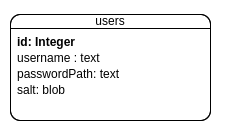
\includegraphics{img/diagrams/erd.png}
    \centering
    \caption{Diagram ERD aplikacji}
    \label{img:erd}
\end{figure}

System w formie bazowej używa tylko jednej tabeli -- \textit{users}, przechowującej:
\begin{itemize}
    \item id -- unikalny identyfikator rekordu
    \item username -- nazwa użytkownika, używana do logowania
    \item passwordPath -- ścieżka do pliku zawierającego formułę $NDB$ kodującą skrót hasła
    \item salt -- \enquote{sól} -- parametr algorytmu uzyskiwania klucza na podstawie frazy hasłowej
\end{itemize}
W przypadku potrzeby przechowywania dodatkowych danych należy dodać do tej tabeli klucze obce łączące użytkowników z~pozostałymi obiektami pozytywnej bazy danych.

W trakcie procedury tworzenia użytkownika generowany jest skrót hasła za pomocą algorytmu PBKDF2 z~użyciem funkcji skrótu SHA-512 oraz losowej soli.
Metoda jest ustawiona na 10000 iteracji i~generuje skrót o~długości 512 bitów. 
Do generacji $NDB$ używany jest algorytm \textit{K-Hidden}, który został wyłoniony na podstawie testów jako najbardziej bezpieczny.
Ponieważ jest to niekompletna metoda generacji konieczne jest zawarcie sumy kontrolnej -- do tego ponownie używana jest funkcja skrótu SHA-512.
Finalny rekord pozytywny jest konkatenacją wyniku funkcji PBKDF2 oraz sumy kontrolnej i~jego długość wynosi 1024 bity.

Tak skonstruowany ciąg bitowy jest kodowany do postaci negatywnej wykorzystując parametry przy których czas rozwiązywania okazał się najdłuższy tj. $p = \{0.7, 0, 0.3\}$, $k = 3$ i~$r = 4.5$.
Następnie powstała $NDB$ jest zapisywana do pliku w formacie \textit{ndb} (zbiór napisów na alfabetem $\{0,1,*\}$), którego ścieżka jest zapisana w kolumnie \textit{passwordPath}. 

\section{Działanie aplikacji}

Aplikacja posiada prosty graficzny interfejs użytkownika składający się z~trzech widoków - logowania, rejestracji oraz panelu użytkownika. Po uruchomieniu widoczne jest okno logowania. Z~tego poziomu można wpisać login i~hasło 
-- jeśli system uzna je za poprawne, to następuje przekierowanie do widoku użytkownika. 

\begin{figure}[h]
    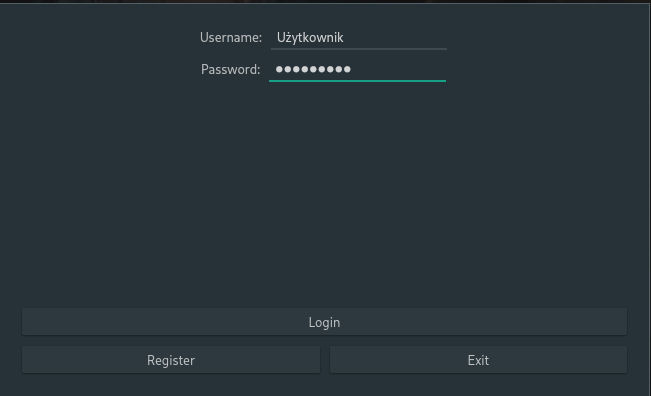
\includegraphics[width=10cm]{img/UI/login.png}
    \centering
    \caption{Panel logowania}
    \label{img:gui-login}
\end{figure}

Po kliknięciu przycisku \textit{Register} na panelu logowania pojawia się widok rejestracji. Tutaj można wprowadzić nowe dane uwierzytelniania i~potwierdzić je ponownie naciskając przycisk \textit{Register} -- jeśli hasło spełnia wymagania,
następuje powrót do widoku loginu, gdzie można uwierzytelnić się nowymi danymi.

\begin{figure}[h]
    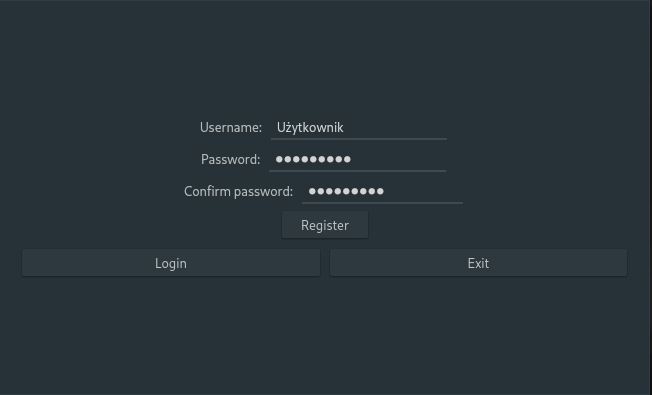
\includegraphics[width=10cm]{img/UI/register.png}
    \centering
    \caption{Panel rejestracji}
    \label{img:gui-register}
\end{figure}

Widok użytkownika oferuje podstawowe funkcje manipulacji kontem. Opcja \textit{Change password} udostępnia możliwość zmiany hasła na nowe oraz \textit{Delete account} powoduje usunięcie wszelkich informacji o~aktywnym użytkowniku.
Po kliknięciu przycisku \textit{Logout} następuje zakończenie sesji i~umożliwia ponowne zalogowanie się na inne konto.

\begin{figure}[h]
    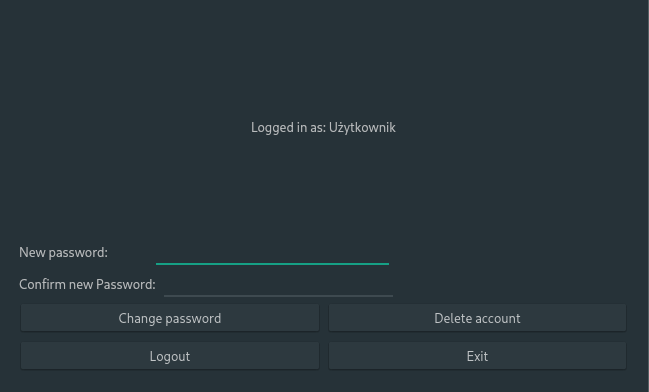
\includegraphics[width=10cm]{img/UI/user.png}
    \centering
    \caption{Panel użytkownika}
    \label{img:gui-user}
\end{figure}

\section{Szczegóły implementacji}
\subsection{Architektura systemu}
Za logikę uwierzytelniania odpowiedzialna jest klasa \textit{AuthenticationManager} oferująca metody do sprawdzenia poprawności danych, tworzenia i~usuwania kont oraz zmiany hasła. Wewnętrznie komunikuje się z klasą \textit{DatabaseAccess} będącą warstwą dostępu do użytej pozytywnej bazy danych.
Obiekty opisujące poszczególne widoki tj. \textit{LoginScreen}, \textit{RegisterScreen} oraz \textit{UserScreen} są w hierarchi poniżej klasy okna głównego -- \textit{MainWindow}. Zbierają dane przekazane przez użytkownika z~odpowiednich pól interfejsu i~tworzą odpowiednie 
zapytania do \textit{AuthenticationManager}.
Przed oddelegowaniem do procedur tworzenia konta i~zmiany hasła dane muszą być zaklasyfikowane jako poprawne za pomocą klasy \textit{PasswordStrengthValidator}, sprawdzającej czy dane hasło spełnia zaprogramowane zasady bezpieczeństwa.
Żeby tworzenie hasła powiodło się musi mieć następujące cechy:
\begin{itemize}
    \item Długość musi wynosić 8 lub więcej znaków
    \item Musi zawierać co najmniej jedną małą literę, jedną wielką literę, jedną cyfre oraz jeden znak specjalny
    \item Nie może być identyczne jak nazwa użytkownika (z pominięciem wielkości liter)
\end{itemize}

\begin{figure}[h]
    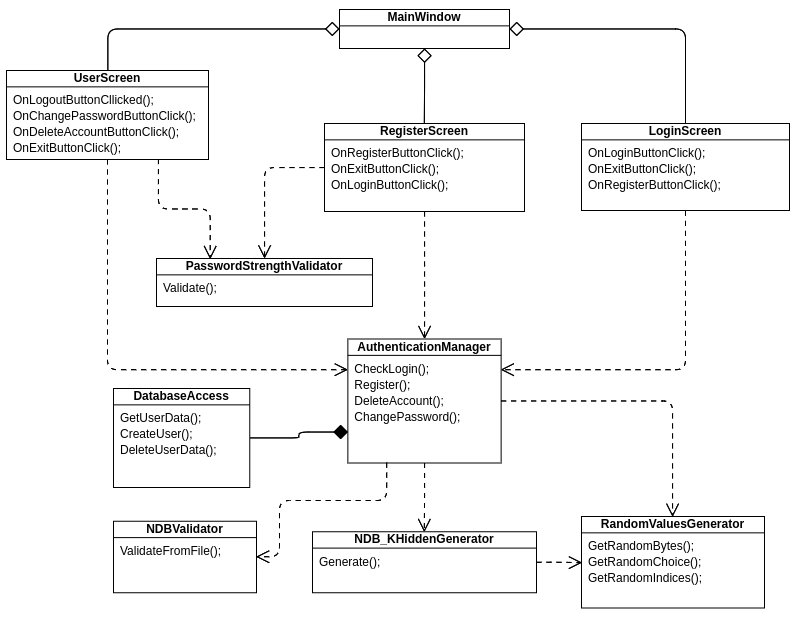
\includegraphics[width = 15.5cm]{img/diagrams/class.png}
    \centering
    \caption{Diagram klas aplikacji}
    \label{img:class}
\end{figure}



\subsection{Algorytm tworzenia użytkownika}
Jeśli dane zostały uznane jako bezpieczne z~punktu widzenia złożoności hasła, obiekty opisujące interfejs tworzą zapytanie o~stworzenie konta. Następnie \textit{AuthenticationManager} sprawdza, czy w bazie nie istnieje użytkownik
o~takiej samej nazwie -- jeśli tak, to proces kończy się porażką i~użytkownik jest o~tym informowany. W innym przypadku tworzony jest rekord $DB$. Sól jest generowana za pomocą klasy pomocniczej \textit{RandomValuesGenerator}.
Następnie tworzony jest obiekt \textit{NDB\_KHiddenGenerator} i~inicjalizowany odpowiednimi parametrami. Powstała $NDB$ jest generowana do pliku i~jej ścieżka oraz pozostałe dane umieszczane są w bazie relacyjnej.
\begin{figure}[h]
    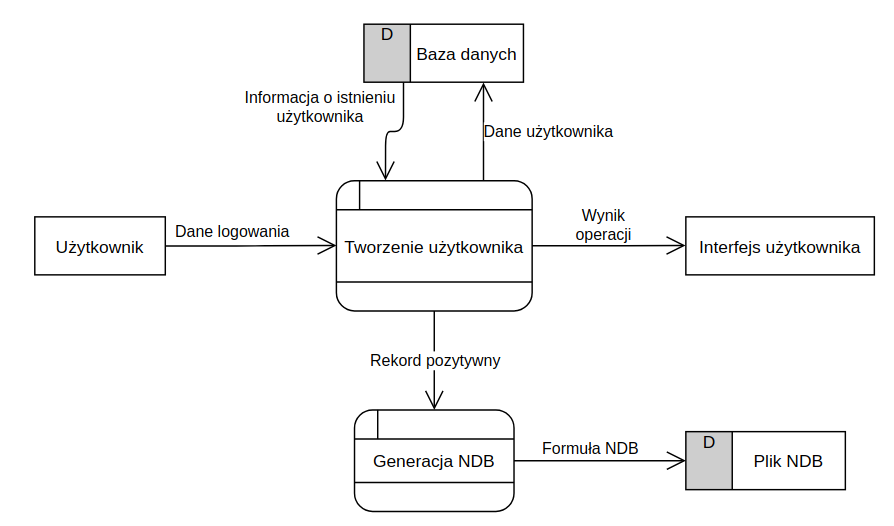
\includegraphics[width = 15.5cm]{img/diagrams/dfdregister.png}
    \centering
    \caption{Diagram przepływu danych w algorytmie tworzenia użytkownika}
    \label{img:dfd-register}
\end{figure}

\subsection{Algorytm uwierzytelniania użytkownika}
Po uzyskaniu od użytkownika loginu i~hasła dane konta są pobierane z~bazy SQLite3, jeżeli istnieją. Następnie wczytywany jest plik $NDB$ za pomocą klasy \textit{NDBValidator}, która sprawdza czy rekord zawierający skrót danego hasła
faktycznie nie pokrywa się z~żadnym rekordem negatywnym. W takim przypadku \textit{AuthenticationManager} zwraca sygnał, że użytkownik powinien mieć dostęp do danych.

\begin{figure}[h]
    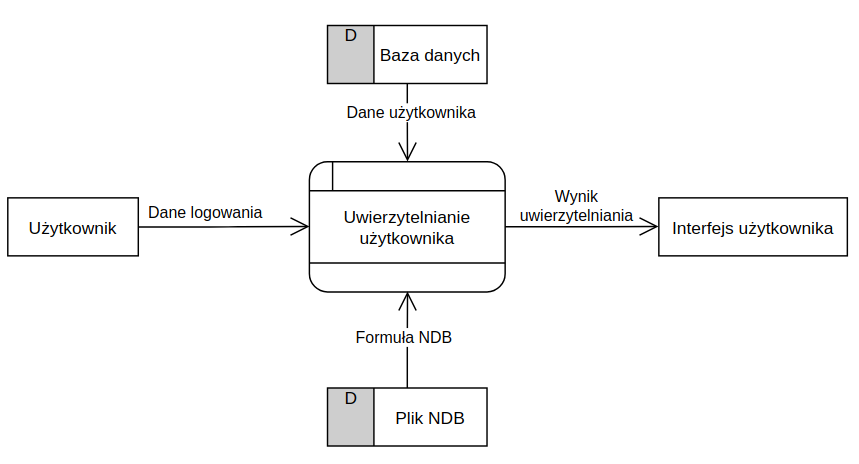
\includegraphics[width = 15.5cm]{img/diagrams/dfdlogin.png}
    \centering
    \caption{Diagram przepływu danych w algorytmie logowania}
    \label{img:dfd-login}
\end{figure}


\subsection{Algorytm zmiany hasła}
Po otrzymaniu zapytania o~zmianę hasła pobierana jest ścieżka do pliku dotychczasowej $NDB$ i~generowany jest nowy rekord $DB$ na podstawie algorytmu tworzenia użytkownika. Następnie inicjalizowany jest nowy obiekt generatora $NDB$ i~wynik jego działania zastępuje
dotychczasowe hasło w postaci negatywnej.

\begin{figure}[h]
    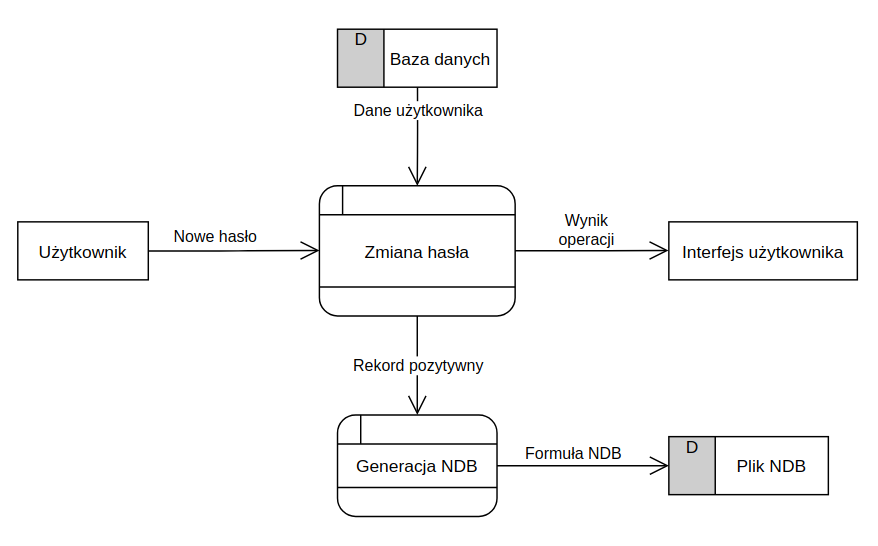
\includegraphics[width = 15.5cm]{img/diagrams/dfdchange.png}
    \centering
    \caption{Diagram przepływu danych w algorytmie zmiany hasła}
    \label{img:dfd-change}
\end{figure}


% !TeX spellcheck = pl_PL
\chapter{Testy algorytmów}
\label{chp:tests}
%%%%%%%%%%%%%%%%%%%%%%%%%%%%%%%%%%%%%%%%%%%%%%%%%%%%%%%%%%%%%%%%%%%%%%%%%%%%%%%%%%%%%%%%%%%%%%%%%%%%%%%%%%%%%%%%%%%%%%%%%%%%%%%%%%%%%%%%%%%%%%%%%%%%%%%%%%%%%%%%%%%%%%%%%%%%%%%%%%%%%%%%%%%%%%%%%%%%%%%%%%%%%%%%%%%%%%%%%%%%%%%%%%%%
\section{Opis testowania za pomocą solwerów SAT}
%%%%%%%%%%%%%%%%%%%%%%%%%%%%%%%%%%%%%%%%%%%%%%%%%%%%%%%%%%%%%%%%%%%%%%%%%%%%%%%%%%%%%%%%%%%%%%%%%%%%%%%%%%%%%%%%%%%%%%%%%%%%%%%%%%%%%%%%%%%%%%%%%%%%%%%%%%%%%%%%%%%%%%%%%%%%%%%%%%%%%%%%%%%%%%%%%%%%%%%%%%%%%%%%%%%%%%%%%%%%%%%%%%%%


Do testów $NDB$ użyte zostały zChaff oraz WalkSAT -- najbardziej popularny solwer kompletny i~niekompletny.
Wszystkie testy zostały przeprowadzone za pomocą aplikacji konsolowej napisanej w języku C++17 z~wykorzystaniem
biblioteki \textit{boost} do wygenerowania opcji programu i~ułatwienia operacji na napisach.

\begin{figure}[h]
    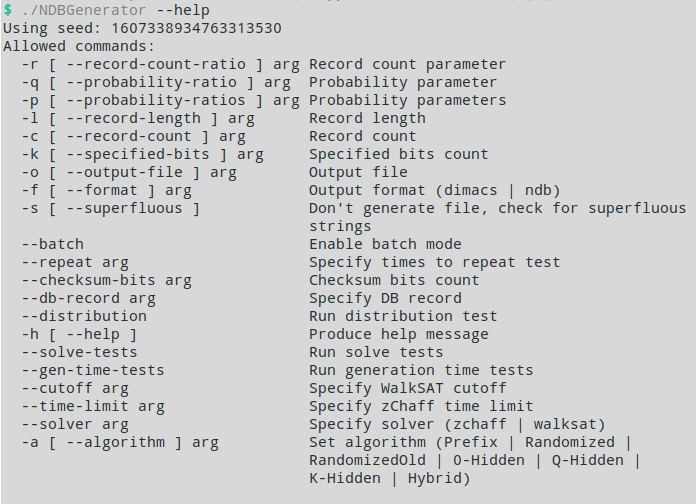
\includegraphics[width=15cm]{img/NDBGeneratorHelp.png}
    \centering
    \caption{Opcje aplikacji testującej}
    \label{img:NDBGenHelp}
\end{figure}

Przy wywołaniu programu użytkownik może ustawić szereg wartości dla każdego dostępnego parametru i~wybrać pożądany algorytm oraz typ testu.
Aplikacja następnie generuję losową $NDB$ dla każdej kombinacji parametrów, przeprowadza test oraz zapisuje wynik do pliku w formacie csv.

Możliwe jest także wygenerowanie pliku Negatywnej Bazy Danych w formacie \textit{ndb} tj. plik tekstowy zawierający napisy
nad alfabetem $\{0,1,*\}$, lub \textit{dimacs} - domyślnym formacie wykorzystywanym przez solwery SAT.
\begin{lstlisting}[caption={Przykładowy plik formatu \textit{dimacs}\\Zawartość składa się z~komentarzy (linie zaczynające się znakiem \enquote{c}), definicji problemu (linia zaczynająca się znakiem \enquote{p})
i klauzul logicznych.\\ W tym przypadku opisywany jest problem CNF o~trzech zmiennych i~dwóch klauzulach reprezentujący formułę $(\neg x_1 \lor \neg x_3) \land (\neg x_2 \lor x_3 \lor x_1) $.},captionpos=b]

c Przykładowy plik cnf
p cnf 3 2
-1 -3 0
-2 3 1 0 
\end{lstlisting}

Aplikacja jest zintegrowana z~napisaną w języku C implementacją algorytmu WalkSAT przedstawioną przez Uniwersytet w Rochester \cite{walksat-implementation}
oraz implementacją zChaff w języku C++ udostępnioną przez Uniwersytet w Princeton \cite{zchaff-implementation}.

Oba programy posiadają interfejs wiersza poleceń i~przyjmują pliki w formacie \textit{dimacs}. Z~powodu potrzeby testowania
znacznej ilości automatycznie generowanych formuł aplikacja testowa wywołuje procedury rozwiązujące bezpośrednio z~kodu.
W przypadku solwera zChaff wymagane było jedynie załączenie pliku nagłówkowego i~zalinkowaniu zbudowanej biblioteki, jednak przy integrowaniu
solwera WalkSAT konieczna była minimalna modyfikacja plików źródłowych w celu umożliwienia wywołania głównej funkcji oraz zresetowania
stanu po próbie rozwiązania każdej formuły.


%%%%%%%%%%%%%%%%%%%%%%%%%%%%%%%%%%%%%%%%%%%%%%%%%%%%%%%%%%%%%%%%%%%%%%%%%%%%%%%%%%%%%%%%%%%%%%%%%%%%%%%%%%%%%%%%%%%%%%%%%%%%%%%%%%%%%%%%%%%%%%%%%%%%%%%%%%%%%%%%%%%%%%%%%%%%%%%%%%%%%%%%%%%%%%%%%%%%%%%%%%%%%%%%%%%%%%%%%%%%%%%%%%%%
\section{Rozkład statystyczny $NDB$}
%%%%%%%%%%%%%%%%%%%%%%%%%%%%%%%%%%%%%%%%%%%%%%%%%%%%%%%%%%%%%%%%%%%%%%%%%%%%%%%%%%%%%%%%%%%%%%%%%%%%%%%%%%%%%%%%%%%%%%%%%%%%%%%%%%%%%%%%%%%%%%%%%%%%%%%%%%%%%%%%%%%%%%%%%%%%%%%%%%%%%%%%%%%%%%%%%%%%%%%%%%%%%%%%%%%%%%%%%%%%%%%%%%%%

Negatywne Bazy Danych wygenerowane przez poszczególne algorytmy mogą różnić się znacząco. Jednym ze sposobów ich porównania jest przedstawienie prawdopodobieństw pojawienia się określonych typów literałów
w~rekordach $NDB$ tj. bitów pokrywających się z~ukrytym napisem, bitów zanegowanych oraz znaków specjalnych \enquote{$*$}. Wynik działania testu rozkładu znajduje się na wykresie \ref{chrt:distribution}.

Algorytm prefiksowy generuje rekordy, w których znak może być odwrócony tylko na jednej pozycji -- zaraz przed serią znaków \enquote{$*$}. Pozostałe możliwości są podzielone równo po połowie.
W~\textit{Randomize\_NDB} znaczna część bitów jest zamieniana na \enquote{$*$}, dodatkowo ustawiana jest niewielka liczba znaków na odwrócone. 

Pozostałe algorytmy generują rekordy składające się z~bardzo niewielu pozycji ustalonych, a~ich wzajemne proporcje są modyfikowalne przez parametry $q$ lub $p$. Analizę ich wpływu na złożoność wygenerowanej bazy przedstawiam 
w~rozdziałach \ref{sec:test-q-hidden}, \ref{sec:test-k-hidden} i~\ref{sec:test-hybrid}.

\begin{figure}
\centering
\begin{tikzpicture}

\begin{axis}[
ybar, axis on top,
height=8cm, width=15cm,
bar width=0.7cm,
ymajorgrids, tick align=inside,
major grid style={draw=white},
%enlarge y limits={value=.1,upper},
ymin=0, ymax=100,
axis x line*=bottom,
axis y line*=right,
y axis line style={opacity=0},
tickwidth=0pt,
enlarge x limits=true,
legend style={
    at={(0.5,-0.2)},
    anchor=north,
    legend columns=-1,
    /tikz/every even column/.append style={column sep=0.5cm}
},
ylabel={Prawdopodobieństwo wystąpienia (\%)},
symbolic x coords={Alg. prefiksowy,Randomize\_NDB,Q-Hidden,K-Hidden,Alg. hybrydowy},
xtick=data,
nodes near coords={
    \pgfmathprintnumber[precision=2]{\pgfplotspointmeta}
}
]
\addplot [draw=none, fill=blue!30] coordinates {
    (Alg. prefiksowy,49.6094)
    (Randomize\_NDB,16.5241) 
    (Q-Hidden,1.27368)
    (K-Hidden,1.25019) 
    (Alg. hybrydowy,1.39286) 
     };
\addplot [draw=none,fill=red!30] coordinates {
    (Alg. prefiksowy,0.78125)
    (Randomize\_NDB,2.67213) 
    (Q-Hidden,1.07007)
    (K-Hidden,1.09356) 
    (Alg. hybrydowy,0.950859) 
    };
\addplot [draw=none, fill=green!30] coordinates {
    (Alg. prefiksowy,49.6094)
    (Randomize\_NDB,80.8037) 
    (Q-Hidden,97.6562)
    (K-Hidden,97.6562) 
    (Alg. hybrydowy,97.6563) 
    };
\legend{Pokrywający się bit,Niepokrywający się bit,Znak $*$}
\end{axis}
\end{tikzpicture}
\caption{Rozkład prawdopodobieństwa pojedynczych pozycji w~wygenerowanych rekordach $NDB$. Dane zgromadzone na podstawie 1000 generacji dla każdego algorytmu.
    Użyte parametry: $l~=~128$, $k~=~3$, $q~=~0.3$, $p~=~\{0.7,~0.2,~0.1\}$, $c~=~1$, $r~=~4.5$}
\label{chrt:distribution}
\end{figure}

%%%%%%%%%%%%%%%%%%%%%%%%%%%%%%%%%%%%%%%%%%%%%%%%%%%%%%%%%%%%%%%%%%%%%%%%%%%%%%%%%%%%%%%%%%%%%%%%%%%%%%%%%%%%%%%%%%%%%%%%%%%%%%%%%%%%%%%%%%%%%%%%%%%%%%%%%%%%%%%%%%%%%%%%%%%%%%%%%%%%%%%%%%%%%%%%%%%%%%%%%%%%%%%%%%%%%%%%%%%%%%%%%%%%
\section{Testy metod weryfikujących poprawność rekordów pozytywnych}
%%%%%%%%%%%%%%%%%%%%%%%%%%%%%%%%%%%%%%%%%%%%%%%%%%%%%%%%%%%%%%%%%%%%%%%%%%%%%%%%%%%%%%%%%%%%%%%%%%%%%%%%%%%%%%%%%%%%%%%%%%%%%%%%%%%%%%%%%%%%%%%%%%%%%%%%%%%%%%%%%%%%%%%%%%%%%%%%%%%%%%%%%%%%%%%%%%%%%%%%%%%%%%%%%%%%%%%%%%%%%%%%%%%%

\label{sec:red-str-test}
Algorytmy generacji $NDB$ \textit{Q-Hidden} oraz \textit{K-Hidden} nie gwarantują pokrycia całego zbioru $U~-~DB$.
Konieczne jest użycie odpowiedniej sumy kontrolnej. Po znalezieniu rozwiązania porównywany jest sufiks rekordu o~określonej
długości z~wynikiem wykorzystanej funkcji na pozostałej części ciągu bitowego. Jeżeli wynik się zgadza to napis jest uznawany za należący
do $DB$.

Zostały przetestowane następujące funkcje sumy kontrolnej:

\begin{itemize}
    \item Bit parzystości (1 bit)
    \item CRC-8 (8 bitów)
    \item CRC-16 (16 bitów)
    \item CRC-32 (32 bity)
    \item MD5 (128 bitów)
\end{itemize}


%%%%%%%%%%%%%%%%%%%%%%%%%%%%%%%%%%%%%%%%%%%%%%%%%%%%%%%%%%%%%%%%%%%%%%%%%%%%%%%%%%%%%%%%%%%%%%%%%%%%%%%%%%%%%%%%%%%%%%%%%%%%%%%%%%%%%%%%%%%%%%%%%%%%%%%%%%%%%%%%%%%%%%%%%%%%%%%%%%%%%%%%%%%%%%%%%%%%%%%%%%%%%%%%%%%%%%%%%%%%%%%%%%%%
\subsection{Wpływ parametrów generacji na liczbę niepożądanych ukrytych ciągów bitowych}
%%%%%%%%%%%%%%%%%%%%%%%%%%%%%%%%%%%%%%%%%%%%%%%%%%%%%%%%%%%%%%%%%%%%%%%%%%%%%%%%%%%%%%%%%%%%%%%%%%%%%%%%%%%%%%%%%%%%%%%%%%%%%%%%%%%%%%%%%%%%%%%%%%%%%%%%%%%%%%%%%%%%%%%%%%%%%%%%%%%%%%%%%%%%%%%%%%%%%%%%%%%%%%%%%%%%%%%%%%%%%%%%%%%%

Celem testu było sprawdzenie, jak zmiana poszczególnych parametrów generacji $NDB$ wpływa na liczbę zakodowanych pozytywnych ciągów różniących się
od zadanego rekordu $s$. 

W celu wyznaczenia dokładnych statystyk, stworzona baza negatywna sprowadzana jest do problemu SAT i~rozwiązywana za pomocą solwera zChaff.  
Po uzyskaniu pojedynczego rozwiązania do bazy wprowadzana jest nowa klauzula CNF -- alternatywa negacji bitów ciągu, która usuwa dany rekord ze zbioru $DB$. Poprzednie kroki są powtarzane, aż otrzymana formuła będzie niespełnialna. 

Rezultatem działania tej procedury jest pełny zbiór $DB$ dla danej bazy, którego wielkość (z wyłączeniem oryginalnego rekordu) jest szukaną miarą.

\begin{figure}[!h]
\begin{subfigure}{0.5\textwidth}
    \captionsetup{width=7cm}
    \centering
    \begin{tikzpicture}[xscale=0.9,yscale=0.9]
    \begin{semilogyaxis}[ylabel = {Średnia liczba nadmiarowych napisów}, xlabel={r}]
        \addplot[
    color=black,
    mark=*,
    ]
    coordinates {
        (10,0.4)(9.5,0.4)(9,0.4)(8.5,0.6)(8,0.6)(7.5,0.8)(7,0.8)(6.5,0.9)(6,1)(5.5,1)(5,3)(4.5,5)(4,6)(3.5,8)(3,16)(2.5,15)(2,21)(1.5,45)(1,71)
    };
    \addlegendentry{$l=8$}
        \addplot[
    color=black,
    mark=square,
    ]
    coordinates {
        (1,6823)(1.5,2631.6)(2,1092.4)(2.5,408.6)(3,116.8)(3.5,59.2)(4,23.8)(4.5,11.8)(5,8.4)(5.5,4.6)(6,2)(6.5,0.8)(7,0.8)(7.5,0.6)(8,0.6)(8.5,0.6)(9,0.6)(9.5,0.6)(10,0.6)
        
    };
    \addlegendentry{$l=16$}
    \addplot[
    color=black,
    mark=o,
    ]
    coordinates {
       (10,0)(9.5,0.2)(9,0.2)(8.5,0.2)(8,0.3)(7.5,0.6)(7,0.4)(6.5,2.4)(6,4)(5.5,3)(5,3.6)(4.5,33)(4,57.4)(3.5,513.4)(3,598.6)(2.5,9702)(2,42225)(1.5,84702)(1,134222)
               
    };
    \addlegendentry{$l=24$}
    
    
    \end{semilogyaxis}
    \end{tikzpicture}
    \caption{Q-Hidden}
    \label{chrt:no-checksum-q-r}
\end{subfigure}
\begin{subfigure}{0.5\textwidth}
    \centering
    \begin{tikzpicture}[xscale=0.9,yscale=0.9]
    \begin{semilogyaxis}[ylabel = {Średnia liczba nadmiarowych napisów}, xlabel={r}]
    
    \addplot[
    color=black,
    mark=*,
    ]
    coordinates {
        (10,0)(9.5,1)(9,1)(8.5,0)(8,0)(7.5,0)(7,0)(6.5,0)(6,1)(5.5,2)(5,4)(4.5,4.2)(4,4.5)(3.5,7)(3,16)(2.5,21)(2,34)(1.5,47)(1,85)
    };
   \addlegendentry{$l=8$}
    
    \addplot[
    color=black,
    mark=square,
    ]
    coordinates {
        (1,7698.2)(1.5,3085.2)(2,1445.4)(2.5,589.8)(3,244.6)(3.5,94.8)(4,50)(4.5,33.2)(5,15)(5.5,7.2)(6,1.6)(6.5,0.6)(7,0.5)(7.5,0.5)(8,0.5)(8.5,0.5)(9,0.5)(9.5,0.5)(10,0.5)
        };
    \addlegendentry{$l=16$}
    
        \addplot[
    color=black,
    mark=o,
    ]
    coordinates {
        (1,214402)(1.5,45321)(2,33367)(2.5,8249)(3,1061.875)(3.5,274.875)(4,53.5)(4.5,11.5)(5,1.875)(5.5,1.875)(6,0.6)(6.5,0.6)(7,0)(7.5,0.5)(8,0.5)(8.5,0.5)(9,0.5)(9.5,0.5)(10,0.5)        
    };
    \addlegendentry{$l=24$}
    
    \end{semilogyaxis}
    
    \end{tikzpicture}
    \caption{K-Hidden}    
    \label{chrt:no-checksum-k-r}
\end{subfigure}
\caption{Zależność liczby nadmiarowych napisów od współczynnika ilości rekordów $r$~dla $NDB$ 
    wygenerowanych przez algorytm \textit{Q-Hidden} i~\textit{K-Hidden} o~parametrach $q=0.4$~/~$p~=~\{0.7, 0.2, 0.1\}$~i~$k~=~3$.}
\end{figure}

\begin{figure}[!h]
    \begin{subfigure}{0.5\textwidth}
    \captionsetup{width=7cm}
    \centering
    \begin{tikzpicture}[xscale=0.9, yscale=0.9]
    \begin{axis}[ylabel = {Mediana liczby nadmiarowych napisów}, xlabel={l}, legend style={at={(0.03,0.8)},anchor=west}
    ]
    
    \addplot[
    color=black,
    mark=diamond,
    ]
    coordinates {
        (8,0.0)(9,1.0)(16,1.0)(17,0.5)(24,0.0)(25,0.0)(32,0.5)(33,0.5)(40,1.0)(41,0.0)(48,1.0)(49,1.0)(56,1.0)(57,1.0)(64,1.0)(65,1.0)(72,1.0)(73,2.0)(80,1.0)(81,1.0)(88,3.0)(89,1.0)(96,2.5)(97,3.0)(104,3.0)(105,3.0)(112,3.0)(113,3.0)(120,3.0)(121,3.0)(128,3.0)(129,3.0)(136,5.0)(137,4.0)(144,5.0)(145,7.0)(152,7.0)(153,7.0)(160,7.0)(161,4.0)(168,7.0)(169,6.0)(176,7.0)(177,7.0)(184,11.0)(185,7.0)(192,11.0)(193,15.0)(200,11.0)(201,15.0)(208,15.0)(209,9.0)(216,15.0)(217,15.0)(224,15.0)(225,15.0)(232,17.0)(233,20.0)(240,23.0)(241,15.0)(248,23.0)(249,24.0)(256,26.0)
        };
    \addlegendentry{$r=6$}
    \addplot[
    color=black,
    mark=square,
    ]
    coordinates {
       (8,1.0)(16,1.0)(24,1.0)(32,1.0)(40,1.0)(48,1.0)(56,3.0)(64,3.0)(72,3.0)(80,3.0)(88,3.0)(96,3.0)(104,3.0)(112,7.5)(120,10.0)(128,7.0)(136,8.0)(144,11.0)(152,27.0)(160,15.0)(168,23.0)(176,47.0)(184,31.0)(192,47.0)(200,47.0)(208,51.0)(216,41.0)(224,47.0)(232,75.0)(240,53.0)(248,95.0)        
    };
    \addlegendentry{$r=5.5$}
    \addplot[
    color=black,
    mark=*,
    ]
    coordinates {
       (8,2.0)(16,4.0)(24,3.0)(32,1.0)(40,3.0)(48,5.0)(56,5.5)(64,11.0)(72,5.5)(80,7.0)(88,16.0)(96,8.0)(104,31.0)(112,35)(120,46.2)(128,72)(136,56)(144,75)(152,70)(160,89)(168,90)(176,97)    
    };
    \addlegendentry{$r=5$}
    
    
    \end{axis}
    \end{tikzpicture}
    \caption{Q-Hidden}
    \label{chrt:no-checksum-q-l}
\end{subfigure}
\begin{subfigure}{0.5\textwidth}
    \centering
    \captionsetup{width=7cm}
    \begin{tikzpicture}[xscale=0.9, yscale=0.9]
    \begin{axis}[ylabel = {Mediana liczby nadmiarowych napisów}, xlabel={l}, legend style={at={(0.03,0.8)},anchor=west}
    ]
    
    \addplot[
    color=black,
    mark=diamond,
    ]
    coordinates {
        (8,1)(12,0)(16,0)(20,0)(24,0)(28,1)(32,0)(36,0)(40,0)(44,1)(48,0)(52,1)(56,1)(60,1)(64,1)(68,1)(72,1)(76,1)(80,2)(84,1)(88,1)(92,1)(96,1)(100,1)(104,1)(108,3)(112,4)(116,3)(120,5)(124,3)(128,3)(132,3)(136,3)(140,5)(144,3)(148,1)(152,7)(156,3)(160,3)(164,4)(168,3)(172,3)(176,7)(180,11)(184,4)(188,7)(192,11)(196,7)(200,11)(204,9)(208,7)(212,11)(216,11)(220,5)(224,9)(228,7)(232,15)(236,9)(240,21)(244,9)(248,11)(252,15)(256,11)
    };
    \addlegendentry{$r=6$}
    \addplot[
    color=black,
    mark=square,
    ]
    coordinates {
(8,1.0)(9,1.0)(16,1.0)(17,1.5)(24,1.0)(25,1.0)(32,2.0)(33,1.0)(40,2.0)(41,2.0)(48,3.0)(49,3.0)(56,3.0)(57,3.0)(64,3.0)(65,3.0)(72,9.0)(73,7.0)(80,8.5)(81,7.0)(88,15.0)(89,7.0)(96,15.0)(97,31.0)(104,9.200000000000001)(105,8.0)(112,10.8)(113,8.4)(120,17.2)(121,9.200000000000001)(128,14.0)(129,29.200000000000003)(136,20.0)(144,18.8)(152,41.2)(160,31.6)(168,63.6)(176,70.0)(184,119.20000000000002)(192,92.4)

    };
    \addlegendentry{$r=5.5$}
    \addplot[
    color=black,
    mark=*,
    ]
    coordinates {
(8,2.9236581246446556)(16,6.193474588181687)(24,5.093895146368432)(32,1.4619326593310134)(40,5.576685112724268)(48,8.161785147204432)(56,8.521623408052468)(64,19.566637667041633)(72,7.7481427493677755)(80,13.238121928366919)(88,27.81180625303228)(96,13.222375917015809)(104,56.487992817647)(112,82)(120,94.2)(128,98)(136,94)(144,102)(152,121)(160,140)
    };
    \addlegendentry{$r=5$}
    \end{axis}
    \end{tikzpicture}
    \caption{K-Hidden}
    \label{chrt:no-checksum-k-l}
\end{subfigure}
\caption{Zależność liczby nadmiarowych napisów od długości rekordu $l$~dla $NDB$
    wygenerowanych przez algorytm \textit{Q-Hidden} i~\textit{K-Hidden} o~parametrach $q~=~0.3$~/~$p~=~\{0.7,~0.2,~0.1\}$~i~$k~=~3$.}
\end{figure}

Jak wynika z~testów, których wyniki są umieszczone na wykresach \ref{chrt:no-checksum-q-r} i~\ref{chrt:no-checksum-k-r}
liczba nadmiarowych napisów ukrytych maleje wykładniczo wraz z~wzrostem parametru $r$. Dla liczby rekordów pięciokrotnie większej niż długość napisu
zachowują się jedynie pojedyncze niepożądane ciągi. 

Długość rekordu także ma znaczny wpływ na ich liczbę, zwłaszcza dla małych wartości $r$, jednak przeprowadzanie testów dla całego przedziału $r \in [1, 10]$ dla $l > 24$ jest niepraktyczne ze względu na złożoność obliczeniową. 

Wraz ze wzrostem parametru $r$ zwiększa się wartość progowa długości rekordu, której przekroczenie powoduje znaczne zwiększenie tempa przyrostu liczby napisów nienależących do $DB$.
Jak wynika z~wykresów \ref{chrt:no-checksum-q-l} i~\ref{chrt:no-checksum-k-l} dla wartości $r=5$ nachylenie funkcji wzrasta przy $l \approx 100$ a~dla $r=5.5$ przy $l \approx 150$.

Z powodu znacznej fluktuacji wyników aby przedstawić dokładną tendencję konieczne było zastosowanie mediany zamiast wartości średniej. 

Negatywne Bazy Danych wygenerowane przez algorytm \textit{Q-Hidden} i~\textit{K-Hidden} nie różnią się znacząco od siebie w~kontekście tego testu.

%%%%%%%%%%%%%%%%%%%%%%%%%%%%%%%%%%%%%%%%%%%%%%%%%%%%%%%%%%%%%%%%%%%%%%%%%%%%%%%%%%%%%%%%%%%%%%%%%%%%%%%%%%%%%%%%%%%%%%%%%%%%%%%%%%%%%%%%%%%%%%%%%%%%%%%%%%%%%%%%%%%%%%%%%%%%%%%%%%%%%%%%%%%%%%%%%%%%%%%%%%%%%%%%%%%%%%%%%%%%%%%%%%%%
\subsection{Skuteczność funkcji sum kontrolnych}
%%%%%%%%%%%%%%%%%%%%%%%%%%%%%%%%%%%%%%%%%%%%%%%%%%%%%%%%%%%%%%%%%%%%%%%%%%%%%%%%%%%%%%%%%%%%%%%%%%%%%%%%%%%%%%%%%%%%%%%%%%%%%%%%%%%%%%%%%%%%%%%%%%%%%%%%%%%%%%%%%%%%%%%%%%%%%%%%%%%%%%%%%%%%%%%%%%%%%%%%%%%%%%%%%%%%%%%%%%%%%%%%%%%%
\begin{figure}[!h]
    \centering
    \begin{tikzpicture}
    \begin{semilogyaxis}[ylabel = {Średnia liczba nadmiarowych napisów}, xlabel={r}, legend style={font=\small}]
    
    
    \addplot[
    color=black,
    mark=diamond,
    ]
    coordinates {
        (5.0,275.17391304347825)(5.1,236.6)(5.2,239.5)(5.3,198.666666666666664)(5.4,207.53333333333333)(5.5,57.6)(5.6,21.933333333333334)(5.7,24.8)(5.8,19.533333333333335)(5.9,15.933333333333334)(6.0,13.266666666666667)(6.1,12.2)(6.2,10.866666666666667)(6.3,4.7)(6.4,4.7666666666666666)(6.5,3.86666666666667)(6.6,3.6)(6.7,2.5)(6.8,2.3)(6.9,2.2)(7.0,1.5)
    };
    \addlegendentry{Bez sumy kont.}
    \addplot[
    color=black,
    mark=square,
    ]
    coordinates {
       (5.0,106.34782608695652)(5.1,67.6)(5.2,83.35714285714286)(5.3,119.8)(5.4,55.13333333333333)(5.5,10.933333333333334)(5.6,12.6)(5.7,11.766666666666667)(5.8,3.8333333333333335)(5.9,5.233333333333333)(6.0,5)(6.1,4.566666666666667)(6.2,4.1666666666666667)(6.3,2.433333333333333)(6.4,3.1)(6.5,1.4333333333333333)(6.6,1.3)(6.7,1.49333333333333333)(6.8,1.3666666666666667)(6.9,0.7)(7.0,0.5)        
    };
    \addlegendentry{Bit parzystości}
    \addplot[
    color=black,
    mark=*,
    ]
    coordinates {
        (5.0,1.2333333333333334)(5.1,0.5)(5.2,0.4)(5.3,0.5)(5.4,0)(5.5,0.13793103448275862)(5.6,0.16666666666666666)(5.7,0.03333333333333333)(5.8,0.1)(5.9,0)(6.0,0.03333333333333333)(6.1,0.03333333333333333)(6.2,0.03333333333333333)(6.3,0)(6.4,0)(6.5,0)(6.6,0)(6.7,0.03333333333333333)(6.8,0)(6.9,0)(7.0,0.03333333333333333)
   };
    \addlegendentry{CRC-8}
    \addplot[
    color=black,
    mark=o,
    ]
    coordinates {
        (5.0,0.1)(5.1,0.05)(5.2,0.03)(5.3,0)(5.4,0)(5.5,0)(5.6,0)(5.7,0)(5.8,0)(5.9,0)(6.0,0)(6.1,0)(6.2,0)(6.3,0)(6.4,0)(6.5,0)(6.6,0)(6.7,0)(6.8,0)(6.9,0)(7.0,0)
    };
    \addlegendentry{CRC-16}
    
    \end{semilogyaxis}
    \end{tikzpicture}
    \caption{Zależność liczby  nadmiarowych napisów od współczynnika ilości rekordów $r$~i~metody sumy kontrolnej.
        Dla każdego punktu na wykresie wygenerowane zostało 10 $NDB$ przez algorytm \textit{K-Hidden} o~parametrach  $p~=~\{0.7, 0.2, 0.1\}$~i~$k~=~3$ 
        oraz 10 przez \textit{Q-Hidden}
        o~parametrach $q=0.3$ i~$k=3$. Dla CRC-32 oraz MD5 nie zostały wykryte żadne nadmiarowe napisy.
    }
    \label{chrt:no-checksum-k-l}
\end{figure}
Wynik porównania różnych metod sumy kontrolnej pokrywa się z intuicją, według której każdy dodatkowy bit zmniejsza liczbę ciągów bitowych
nienależących do $DB$ o~połowę. Wynika z~tego, że funkcja skrótu o~długości 32 bitów, jest wystarczająca, żeby zapewnić spójność bazy danych
przy zastosowaniach w~których nie trzeba przechowywać danych krytycznych.

W systemach uwierzytelniania zalecane jest jednak użycie większej wartości w~celu zredukowania szansy konfliktu danych do praktycznie niemożliwej.  



%%%%%%%%%%%%%%%%%%%%%%%%%%%%%%%%%%%%%%%%%%%%%%%%%%%%%%%%%%%%%%%%%%%%%%%%%%%%%%%%%%%%%%%%%%%%%%%%%%%%%%%%%%%%%%%%%%%%%%%%%%%%%%%%%%%%%%%%%%%%%%%%%%%%%%%%%%%%%%%%%%%%%%%%%%%%%%%%%%%%%%%%%%%%%%%%%%%%%%%%%%%%%%%%%%%%%%%%%%%%%%%%%%%%
\section{Testy algorytmów generacji $NDB$}
%%%%%%%%%%%%%%%%%%%%%%%%%%%%%%%%%%%%%%%%%%%%%%%%%%%%%%%%%%%%%%%%%%%%%%%%%%%%%%%%%%%%%%%%%%%%%%%%%%%%%%%%%%%%%%%%%%%%%%%%%%%%%%%%%%%%%%%%%%%%%%%%%%%%%%%%%%%%%%%%%%%%%%%%%%%%%%%%%%%%%%%%%%%%%%%%%%%%%%%%%%%%%%%%%%%%%%%%%%%%%%%%%%%%

W~tym rozdziale opisuję wyniki testów poszczególnych algorytmów pod kątem odporności na odwrócenie. 
W~tym celu pokazuję jak zmiana parametrów wpływa na czas znalezienia pierwszego rozwiązania przez solwery SAT i~na wymaganą do tego liczbę operacji.

Pojedynczą operacją w solwerze zChaff jest decyzja -- polega na wybraniu niewykorzystanej zmiennej i~przypisaniu określonej wartości logicznej \cite{chaff}. 
W~przypadku WalkSAT operacją jest odwrócenie przypisań (\textit{flip}) opisane w rozdziale \ref{sec:gsat}.

Dodatkowo przedstawiam złożoności czasowe samego etapu generacji w zależności od ustawionych parametrów.

%%%%%%%%%%%%%%%%%%%%%%%%%%%%%%%%%%%%%%%%%%%%%%%%%%%%%%%%%%%%%%%%%%%%%%%%%%%%%%%%%%%%%%%%%%%%%%%%%%%%%%%%%%%%%%%%%%%%%%%%%%%%%%%%%%%%%%%%%%%%%%%%%%%%%%%%%%%%%%%%%%%%%%%%%%%%%%%%%%%%%%%%%%%%%%%%%%%%%%%%%%%%%%%%%%%%%%%%%%%%%%%%%%%%
\subsection{Algorytm prefiksowy}
%%%%%%%%%%%%%%%%%%%%%%%%%%%%%%%%%%%%%%%%%%%%%%%%%%%%%%%%%%%%%%%%%%%%%%%%%%%%%%%%%%%%%%%%%%%%%%%%%%%%%%%%%%%%%%%%%%%%%%%%%%%%%%%%%%%%%%%%%%%%%%%%%%%%%%%%%%%%%%%%%%%%%%%%%%%%%%%%%%%%%%%%%%%%%%%%%%%%%%%%%%%%%%%%%%%%%%%%%%%%%%%%%%%%
Algorytm prefiksowy jest bardzo prostą metodą generacji $NDB$, dlatego odwrócenie rezultatu jej działania nie stanowi problemu. Sposób na uzyskanie zbioru $DB$ bez użycia solwera SAT został zaprezentowany w~algorytmie \ref{alg:prefix-reverse}.
Generacja ma stosunkową niską złożoność czasową, nawet dla bardzo długich ciągów, jednak zawarcie wielu rekordów $DB$ może ją znacznie spowolnić\footnote{Testy czasowe algorytmów zostały przeprowadzone przez wyliczenie czasu procesora podczas działania określonej procedury na komputerze wyposażonym w~procesor Intel i5-7200U 3.1 GHz i~16 GB pamięci RAM.}.

\begin{figure}[!htb]
    \centering
    \begin{tikzpicture}
    \begin{axis}[ylabel={Średni czas generacji [s]}, xlabel={l}, legend style={at={(0.03,0.8)}, anchor=west}]
    \addplot[
    color=black,
    mark=square,
    ]
    coordinates {
        (16,0)(32,0)(48,0)(64,0)(80,0)(96,0)(112,0)(128,0.001)(144,0.001)(160,0.001)(176,0.001)(192,0.004)(208,0.005)(224,0.004)(240,0.005)(256,0.007)(272,0.006)(288,0.006)(304,0.006)(320,0.007)(336,0.008)(352,0.012)(368,0.01)(384,0.009)(400,0.011)(416,0.015)(432,0.012)(448,0.015)(464,0.018)(480,0.014)(496,0.012)(512,0.016)(528,0.02)(544,0.015)(560,0.022)(576,0.018)(592,0.028)(608,0.026)(624,0.021)(640,0.029)(656,0.027)(672,0.026)(688,0.033)(704,0.032)(720,0.034)(736,0.032)(752,0.031)(768,0.036)(784,0.036)(800,0.04)(816,0.039)(832,0.04)(848,0.037)(864,0.041)(880,0.042)(896,0.043)(912,0.047)(928,0.048)(944,0.052)(960,0.054)(976,0.059)(992,0.057)(1008,0.061)(1024,0.057)
    };
    \addlegendentry{$c = 1$}
    \addplot[
    color=black,
    mark=diamond,
    ]
    coordinates {
        (16,0)(32,0.001)(48,0.002)(64,0.003)(80,0.004)(96,0.008)(112,0.011)(128,0.013)(144,0.017)(160,0.022)(176,0.025)(192,0.028)(208,0.029)(224,0.037)(240,0.042)(256,0.044)(272,0.05)(288,0.055)(304,0.061)(320,0.067)(336,0.055)(352,0.049)(368,0.051)(384,0.055)(400,0.06)(416,0.063)(432,0.07)(448,0.083)(464,0.076)(480,0.082)(496,0.086)(512,0.096)(528,0.115)(544,0.115)(560,0.117)(576,0.116)(592,0.129)(608,0.128)(624,0.139)(640,0.143)(656,0.151)(672,0.152)(688,0.166)(704,0.175)(720,0.178)(736,0.184)(752,0.195)(768,0.219)(784,0.208)(800,0.22)(816,0.226)(832,0.239)(848,0.249)(864,0.254)(880,0.267)(896,0.267)(912,0.279)(928,0.303)(944,0.301)(960,0.319)(976,0.319)(992,0.333)(1008,0.363)(1024,0.356)
    };
    \addlegendentry{$c = 10$}
    \addplot[
    color=black,
    mark=x,
    ]
    coordinates{
(16,0.004)(32,0.012)(48,0.036)(64,0.054)(80,0.065)(96,0.094)(112,0.123)(128,0.148)(144,0.178)(160,0.213)(176,0.222)(192,0.238)(208,0.295)(224,0.332)(240,0.39)(256,0.43)(272,0.475)(288,0.452)(304,0.483)(320,0.68)(336,0.752)(352,0.816)(368,0.968)(384,0.826)(400,1.113)(416,1.228)(432,1.356)(448,1.456)(464,1.574)(480,1.521)(496,1.593)(512,1.568)(528,1.556)(544,1.678)(560,1.677)(576,1.713)(592,1.79)(608,1.547)(624,1.58)(640,1.466)(656,1.812)(672,1.877)(688,1.905)(704,1.779)(720,1.791)(736,1.874)(752,1.948)(768,2.042)(784,2.139)(800,2.368)(816,2.295)(832,2.364)(848,2.499)(864,2.595)(880,2.67)(896,2.739)(912,2.838)(928,2.999)(944,3.118)(960,3.152)(976,3.246)(992,3.587)(1008,3.54)(1024,3.57)
    };
     \addlegendentry{$c = 100$}
    \end{axis}
    \end{tikzpicture}
    \caption{Zależność czasu generacji $NDB$ za pomocą algorytmu prefiksowego od długości kodowanego ciągu.}
    \label{chrt:prefix-timegen}
\end{figure}

\begin{figure}[!htb]
\begin{subfigure}{0.5\textwidth}
    \captionsetup{width=7cm}
    \centering
    \begin{tikzpicture}[xscale=0.9,yscale=0.9]
    \begin{axis}[ylabel={Średni czas odwracania $NDB$ [ms]}, xlabel={l}, legend style={at={(0.03,0.8)}, anchor=west}]
    \addplot[
    color=black,
    mark=square,
    ]
    coordinates {
        (16,1)(32,1)(48,1)(64,1)(80,1)(96,1)(112,1)(128,1)(144,1)(160,1)(176,1)(192,1)(208,1)(224,1)(240,1)(256,1)(272,1)(288,1)(304,1)(320,1)(336,1)(352,1)(368,1)(384,1)(400,1)(416,1)(432,1)(448,1)(464,1)(480,1)(496,1)(512,1)(528,1)(544,1)(560,1)(576,1)(592,1)(608,1)(624,1)(640,1)(656,1)(672,1)(688,1)(704,1)(720,1)(736,1)(752,1)(768,1)(784,1)(800,1)(816,1)(832,1)(848,1)(864,1)(880,1)(896,1)(912,1)(928,1)(944,1)(960,1)(976,1)(992,1)(1008,1)(1024,1)
    };
    \addlegendentry{$c = 1$}
    \addplot[
    color=black,
    mark=diamond,
    ]
    coordinates {
        (16,0)(32,0)(48,0)(64,0)(80,0.04)(96,0.02)(112,0.1)(128,0.18)(144,0.3)(160,0.34)(176,0.64)(192,0.92)(208,0.86)(224,1.08)(240,1)(256,1.68)(272,2)(288,1.66)(304,2.2)(320,2.2)(336,2.84)(352,2.64)(368,3.3)(384,3.56)(400,3.92)(416,4.18)(432,4.18)(448,4.5)(464,5.24)(480,5.66)(496,5.48)(512,6.46)(528,6.36)(544,7.08)(560,8.76)(576,9.84)(592,8.72)(608,10.02)(624,11.24)(640,10.14)(656,11.26)(672,11.32)(688,13.46)(704,13.1)(720,14.18)(736,14.18)(752,17.26)(768,17.98)(784,19.24)(800,17.64)(816,18.58)(832,22.26)(848,20.42)(864,21.3)(880,21.42)(896,24.4)(912,25.52)(928,25.16)(944,24.98)(960,26.32)(976,27.24)(992,29.58)(1008,32.4)(1024,31.4)
    };
    \addlegendentry{$c = 10$}
    \addplot[
    color=black,
    mark=x,
    ]
    coordinates{
        (16,0.0)(32,0.0)(48,0.0)(64,0.0)(80,0.1)(96,0.1)(112,0.4)(128,1.0)(144,1.2)(160,1.6)(176,2.5)(192,3.7)(208,3.4)(224,5.1)(240,5.3)(256,5.8)(272,8.2)(288,9.2)(304,9.2)(320,9.4)(336,11.4)(352,11.8)(368,13.6)(384,15.3)(400,17.0)(416,17.3)(432,19.4)(448,20.8)(464,21.2)(480,21.5)(496,23.1)(512,24.4)(528,27.2)(544,29.7)(560,33.5)(576,30.2)(592,32.9)(608,36.0)(624,40.7)(640,40.2)(656,41.6)(672,40.3)(688,42.6)(704,46.5)(720,48.5)(736,54.7)(752,50.7)(768,54.2)(784,60.5)(800,68.3)(816,68.9)(832,69.9)(848,69.3)(864,66.5)(880,66.4)(896,84.8)(912,80.3)(928,84.7)(944,90.8)(960,98.7)(976,102.2)(992,102.6)(1008,94.8)(1024,91.1)
        
    };
    \addlegendentry{$c = 100$}
    \end{axis}
    \end{tikzpicture}
    \caption{zChaff}
    \label{chrt:prefix-time}
\end{subfigure}
\begin{subfigure}{0.5\textwidth}
    \captionsetup{width=7cm}
    \centering
    \begin{tikzpicture}[xscale=0.9,yscale=0.9]
    \begin{axis}[ylabel={Średni czas odwracania $NDB$ [min]}, xlabel={l}, legend style={at={(0.03,0.8)}, anchor=west}]
    \addplot[
    color=black,
    mark=square,
    ]
    coordinates {
(8,0.0)(9,0.0)(10,0.0)(11,0.0)(12,0.0)(13,0.0)(14,0.0)(15,0.0)(16,0.0)(17,0.00016666666666666666)(18,0.0003333333333333333)(19,0.0005)(20,0.0003333333333333333)(21,0.0018333333333333333)(22,0.0035)(23,0.006)(24,0.007166666666666667)(25,0.023666666666666666)(26,0.043000000000000003)(27,0.105)(28,0.36733333333333335)(29,0.47733333333333333)(30,0.9963333333333334)(31,1.4383333333333332)(32,2.0563333333333333)(33,5.598166666666667)(34,5.183833333333333)(35,11.835666666666667)(36,11.336500000000001)(37,16.208833333333335)(38,21.139833333333335)(39,18.578)
        
    };
    \addlegendentry{$c = 1$}
    \addplot[
    color=black,
    mark=diamond,
    ]
    coordinates {
    (8,0.0)(9,0.0)(10,0.0)(11,0.0)(12,0.0)(13,0.0)(14,0.0)(15,0.0)(16,4.9999999999999996e-06)(17,2.1666666666666667e-05)(18,2.6666666666666667e-05)(19,6e-05)(20,3e-05)(21,8.5e-05)(22,0.00036)(23,0.0008299999999999999)(24,0.0019133333333333333)(25,0.006466666666666667)(26,0.005385)(27,0.019340000000000003)(28,0.011043333333333332)(29,0.04821166666666667)(30,0.06841)(31,0.2652366666666667)(32,0.458505)(33,1.1550049999999998)(34,3.2571483333333333)(35,2.5153966666666667)(36,5.838048333333333)(37,11.533615)(38,16.259691666666665)(39,28.399173333333334)
        
    };
    \addlegendentry{$c = 10$}
    \addplot[
    color=black,
    mark=x,
    ]
    coordinates{
(8,0.0)(9,0.0)(10,0.0)(11,0.0)(12,0.0)(13,0.0)(14,0.0)(15,0.0)(16,0.0)(17,0.0)(18,0.0)(19,0.0)(20,0.0)(21,0.0)(22,0.0)(23,0.0)(24,0.0)(25,0.0)(26,0.0)(27,0.016666666666666666)(28,0.016666666666666666)(29,0.016666666666666666)(30,0.03333333333333333)(31,0.11666666666666667)(32,0.23333333333333334)(33,0.21666666666666667)(34,0.4666666666666667)(35,1.35)(36,0.6833333333333333)(37,6.116666666666666)(38,7.633333333333334)(39,26.8)
   
    };
    \addlegendentry{$c = 100$}
    \end{axis}
    \end{tikzpicture}
    \caption{WalkSAT}
    \label{chrt:prefix-time-w}
\end{subfigure}
\caption{Zależność czasu koniecznego do znalezienia pierwszego rozwiązania od długości ciągu i~liczby rekordów dla $NDB$ wygenerowanych za pomocą algorytmu prefiksowego.}
\end{figure}
\begin{figure}[!htb]
\begin{subfigure}{0.5\textwidth}
    \captionsetup{width=7cm}
    \centering
    \begin{tikzpicture}[xscale=0.9,yscale=0.9]
    \begin{axis}[ylabel={Średnia liczba decyzji}, xlabel={l}, legend style={at={(0.03,0.8)}, anchor=west}]
    \addplot[
    color=black,
    mark=square,
    ]
    coordinates {
        (16,1)(32,1)(48,1)(64,1)(80,1)(96,1)(112,1)(128,1)(144,1)(160,1)(176,1)(192,1)(208,1)(224,1)(240,1)(256,1)(272,1)(288,1)(304,1)(320,1)(336,1)(352,1)(368,1)(384,1)(400,1)(416,1)(432,1)(448,1)(464,1)(480,1)(496,1)(512,1)(528,1)(544,1)(560,1)(576,1)(592,1)(608,1)(624,1)(640,1)(656,1)(672,1)(688,1)(704,1)(720,1)(736,1)(752,1)(768,1)(784,1)(800,1)(816,1)(832,1)(848,1)(864,1)(880,1)(896,1)(912,1)(928,1)(944,1)(960,1)(976,1)(992,1)(1008,1)(1024,1)
    };
    \addlegendentry{$c = 1$}
    \addplot[
    color=black,
    mark=diamond,
    ]
    coordinates {
        (16,6)(32,11)(48,18)(64,30)(80,33)(96,45)(112,64)(128,76)(144,91)(160,95)(176,133)(192,161)(208,158)(224,180)(240,157)(256,230)(272,304)(288,246)(304,275)(320,277)(336,307)(352,282)(368,369)(384,381)(400,405)(416,411)(432,367)(448,415)(464,511)(480,527)(496,459)(512,564)(528,526)(544,517)(560,590)(576,693)(592,587)(608,700)(624,772)(640,582)(656,673)(672,765)(688,762)(704,786)(720,864)(736,724)(752,894)(768,885)(784,1087)(800,832)(816,950)(832,929)(848,826)(864,920)(880,983)(896,1057)(912,1176)(928,1072)(944,1076)(960,1193)(976,1029)(992,997)(1008,1428)(1024,1092)
    };
    \addlegendentry{$c = 10$}
    \addplot[
    color=black,
    mark=x,
    ]
    coordinates{
        (16,7.58)(32,9.62)(48,13.64)(64,15.66)(80,22.82)(96,23.46)(112,30.96)(128,50.46)(144,47.98)(160,55.4)(176,89.12)(192,109.92)(208,110.2)(224,125.62)(240,133.1)(256,130.02)(272,210.14)(288,271.48)(304,215.48)(320,201.76)(336,258.82)(352,260.8)(368,357.52)(384,354.78)(400,440.46)(416,421.7)(432,405.94)(448,465.48)(464,401.04)(480,476.28)(496,454.16)(512,581.14)(528,510.78)(544,681.64)(560,796.68)(576,695.76)(592,767.2)(608,789.98)(624,846.1)(640,916.52)(656,955.34)(672,803.06)(688,866.06)(704,916.28)(720,920.26)(736,1054.3)(752,927.76)(768,1087.86)(784,1146.14)(800,1269.42)(816,1467.4)(832,1312.3)(848,1315.68)(864,1214.8)(880,1125.92)(896,1517.3)(912,1319.9)(928,1467.12)(944,1711.14)(960,1468.12)(976,1841.54)(992,1898)(1008,1406.94)(1024,1507.66)
    };
    \addlegendentry{$c = 100$}
    \end{axis}
    \end{tikzpicture}
    \caption{zChaff}
    \label{chrt:prefix-dec}
\end{subfigure}
\begin{subfigure}{0.5\textwidth}
    \captionsetup{width=7cm}
    \centering
    \begin{tikzpicture}[xscale=0.9,yscale=0.9]
    \begin{axis}[ylabel={Średnia liczba odwróceń przypisań}, xlabel={l}, legend style={at={(0.03,0.8)}, anchor=west}]
    \addplot[
    color=black,
    mark=square,
    ]
    coordinates {
        (8,55.3)(9,241)(10,195.3)(11,815.2)(12,1180.4)(13,1126.7)(14,10774.9)(15,15598.3)(16,23985.7)(17,59097.7)(18,123467.2)(19,277844.4)(20,132090.9)(21,836015.4)(22,1633597.1)(23,2724227.2)(24,3209904.9)(25,10501416.2)(26,18868058.3)(27,45758955.1)(28,160875721.1)(29,207022644.2)(30,420744738.1)(31,600558021.1)(32,861337050.4)(33,2314713706)(34,2129353277)(35,4774140223)(36,4469157089)(37,6275585955)(38,8181380127)(39,7321977601)
        
    };
    \addlegendentry{$c = 1$}
    \addplot[
    color=black,
    mark=diamond,
    ]
    coordinates {
        (8,2)(9,6)(10,11)(11,7)(12,88)(13,71)(14,264)(15,361)(16,936)(17,3559)(18,4443)(19,8583)(20,4456)(21,11667)(22,48127)(23,108675)(24,245824)(25,803191)(26,637552)(27,2266769)(28,1265776)(29,5450840)(30,7557746)(31,28871696)(32,49238112)(33,121225411)(34,338874771)(35,259426141)(36,580907270)(37,1144204637)(38,1496673416)(39,2635124524)
        
    };
    \addlegendentry{$c = 10$}
    \addplot[
    color=black,
    mark=x,
    ]
    coordinates{
        (8,1)(9,1)(10,2)(11,4)(12,4)(13,10)(14,15)(15,20)(16,43)(17,81)(18,212)(19,278)(20,430)(21,1169)(22,2189)(23,4950)(24,16666)(25,19519)(26,34515)(27,109132)(28,177298)(29,256536)(30,333894)(31,1188660)(32,2259196)(33,2063163)(34,4306589)(35,14044363)(36,8204427)(37,55924970)(38,75371771)(39,234689971)
        
    };
    \addlegendentry{$c = 100$}
    \end{axis}
    \end{tikzpicture}
    \caption{WalkSAT}
    \label{chrt:prefix-flips}
\end{subfigure}
\caption{Zależność liczby decyzji/odwróceń przypisań od długości ciągu i~liczby rekordów dla $NDB$ wygenerowanych za pomocą algorytmu prefiksowego.}
\end{figure}


Kompletny solwer zChaff odwraca $NDB$ z~jednym rekordem pozytywnym niemal natychmiast -- dla każdego przypadku została podjęta tylko jedna decyzja.
Przy zawarciu większej liczby napisów znalezienie jednego z~nich staje się trudniejsze, jednak jest to nadal możliwe w~czasie liniowym.

Natomiast dla solwera WalkSAT otrzymana struktura CNF jest problematyczna -- procedura degraduje się w~kierunku losowego przeszukiwania o~wykładniczej złożoności obliczeniowej.
Już dla stu napisów o~długości 40 bitów metoda kończy działanie z~powodu przekroczenia ustawionej na potrzeby testów wartości granicznej 10 prób po $10^9$ odwróceń przypisań.


%%%%%%%%%%%%%%%%%%%%%%%%%%%%%%%%%%%%%%%%%%%%%%%%%%%%%%%%%%%%%%%%%%%%%%%%%%%%%%%%%%%%%%%%%%%%%%%%%%%%%%%%%%%%%%%%%%%%%%%%%%%%%%%%%%%%%%%%%%%%%%%%%%%%%%%%%%%%%%%%%%%%%%%%%%%%%%%%%%%%%%%%%%%%%%%%%%%%%%%%%%%%%%%%%%%%%%%%%%%%%%%%%%%%
\subsection{Algorytm \textit{Randomize\_NDB}}
%%%%%%%%%%%%%%%%%%%%%%%%%%%%%%%%%%%%%%%%%%%%%%%%%%%%%%%%%%%%%%%%%%%%%%%%%%%%%%%%%%%%%%%%%%%%%%%%%%%%%%%%%%%%%%%%%%%%%%%%%%%%%%%%%%%%%%%%%%%%%%%%%%%%%%%%%%%%%%%%%%%%%%%%%%%%%%%%%%%%%%%%%%%%%%%%%%%%%%%%%%%%%%%%%%%%%%%%%%%%%%%%%%%%

Algorytm \textit{Randomize\_NDB} generuje bazy danych o~znacznie większym rozmiarze niż algorytm prefiksowy. Już dla 25 rekordów, każdy o~długości co najmniej 300 bitów, czas trwania procedury generacyjnej przekracza godzinę,
podczas, gdy czas rozwiązywania bazy o~takich parametrach zajmuje solwerowi zChaff niecałe dwie sekundy. Dla ukrywania pojedynczych rekordów procedura działa niewiele wolniej niż algorytm prefiksowy, ale wynikowa $NDB$ będzie bardzo prosta do złamania.

Złożoność otrzymanej bazy zależy głównie od liczby zawartych rekordów pozytywnych, ale czas generacji rośnie dużo szybciej niż trudność problemu SAT. Z~wykresu \ref{chrt:rand-time-z} na pierwszy rzut oka wynika, że dla większych wartości $l$ czas rozwiązania znacznie wzrasta, ale jest to spowodowane
procesem przetwarzania wstępnego solwera zChaff -- dla wszystkich pokazanych przykładów liczba podjętych decyzji nie przekracza pięciu.

Solwer WalkSAT podobnie jak w~przypadku algorytmu prefiksowego wypada znacznie gorzej niż zChaff, jednak tym razem potrafi w~krótkim czasie odwrócić $NDB$ przy $l=100$ i~niewielkiej liczbie rekordów pozytywnych, jednak wraz ze wzrostem $c$ złożoność obliczeniowa zwiększa się drastycznie.

\begin{figure}[!h]
    \centering
    \begin{tikzpicture}
    \begin{axis}[ylabel={Średni czas generacji [min]}, xlabel={l}, legend style={at={(0.03,0.8)}, anchor=west}]
    \addplot[
    color=black,
    mark=square,
    ]
    coordinates {
        (16,0.00025)(32,0.00115)(48,0.003733333333)(64,0.004266666667)(80,0.02518333333)(96,0.05383333333)(112,0.09065)(128,0.04515)(144,0.1289833333)(160,0.1882666667)(176,0.3859666667)(192,0.6316166667)(208,0.82445)(224,0.96245)(240,1.374933333)(256,1.260816667)(272,1.815816667)(288,1.946533333)(304,2.09925)(320,2.791583333)(336,2.594833333)(352,2.902866667)(368,3.498683333)(384,3.981716667)(400,5.058816667)(416,4.78275)(432,6.022966667)(448,5.771866667)(464,9.091316667)(480,10.48951667)(496,12.47911667)(512,14.94341667)

    };
    \addlegendentry{$c = 1$}
    \addplot[
    color=black,
    mark=diamond,
    ]
    coordinates {
        (16,0.00085)(32,0.008866666667)(48,0.04466666667)(64,0.08683333333)(80,0.2802333333)(96,0.4084666667)(112,0.6871833333)(128,0.87305)(144,2.4365)(160,2.942483333)(176,3.691433333)(192,4.55565)(208,7.617466667)(224,6.938716667)(240,7.843183333)(256,11.82141667)(272,21.93571667)(288,26.74303333)(304,30.27935)(320,45.50025)(336,38.72085)(352,45.04981667)(368,50.45198333)(384,57.90636667)(400,62.48886667)(416,70.54368333)(432,88.1753)(448,101.7783333)(464,97.65956667)(480,104.7520167)(496,110.5336667)(512,121.0154167)

    };
    \addlegendentry{$c = 10$}
    \addplot[
    color=black,
    mark=x,
    ]
    coordinates{
        (16,0.003966666667)(32,0.03453333333)(48,0.1718333333)(64,0.3356)(80,1.350816667)(96,1.759766667)(112,2.79695)(128,3.484116667)(144,9.031316667)(160,14.05761667)(176,14.58041667)(192,23.65731667)(208,22.94568333)(224,27.3603)(240,31.40791667)(256,34.77282667)(272,53.32652714)(288,75.21356095)(304,87.10059476)(320,120.6542952)(336,119.2079957)(352,156.0950167)
    };
    \addlegendentry{$c = 25$}
    \end{axis}
    \end{tikzpicture}
    \caption{Zależność czasu generacji $NDB$ za pomocą algorytmu \textit{Randomize\_NDB} od długości kodowanego ciągu.}
    \label{chrt:rand-timegen}
\end{figure}

\begin{figure}[!h]
\begin{subfigure}{0.5\textwidth}
    \captionsetup{width=7cm}
    \centering
    \begin{tikzpicture}[xscale=0.9,yscale=0.9]
    \begin{axis}[ylabel={Średni czas odwracania $NDB$ [s]}, xlabel={l}, legend style={at={(0.03,0.8)}, anchor=west}]
    \addplot[
    color=black,
    mark=square,
    ]
    coordinates {
(16,0)(32,0)(48,0.012)(64,0.001)(80,0.007)(96,0.022)(112,0.033)(128,0.012)(144,0.035)(160,0.054)(176,0.118)(192,0.154)(208,0.169)(224,0.172)(240,0.249)(256,0.277)(272,0.258)(288,0.303)(304,0.333)(320,0.511)(336,0.471)(352,0.507)(368,0.525)(384,0.511)(400,0.74)(416,0.719)(432,0.658)(448,0.781)(464,0.812)(480,1.054)(496,1.355)(512,2.454)
    };
    \addlegendentry{$c = 1$}
    \addplot[
    color=black,
    mark=diamond,
    ]
    coordinates {
(16,0)(32,0.001)(48,0.006)(64,0.009)(80,0.03)(96,0.058)(112,0.062)(128,0.099)(144,0.151)(160,0.162)(176,0.239)(192,0.26)(208,0.337)(224,0.358)(240,0.472)(256,0.893)(272,0.859)(288,0.95)(304,1.225)(320,1.205)(336,1.354)(352,1.29)(368,1.397)(384,1.495)(400,1.523)(416,1.688)(432,1.79)(448,1.76)(464,2.115)(480,2.456)(496,2.774)(512,2.662)

    };
    \addlegendentry{$c = 10$}
    \addplot[
    color=black,
    mark=x,
    ]
    coordinates{
(16,0)(32,0.003)(48,0.015)(64,0.022)(80,0.094)(96,0.08)(112,0.182)(128,0.15)(144,0.357)(160,0.494)(176,0.435)(192,0.684)(208,0.785)(224,0.952)(240,0.888)(256,1.150571429)(272,1.224107143)(288,1.297642857)(304,1.371178571)(320,1.544)(336,1.718)(352,1.821)


    };
    \addlegendentry{$c = 25$}
    \end{axis}
    \end{tikzpicture}
    \caption{zChaff}
    \label{chrt:rand-time-z}
\end{subfigure}
\begin{subfigure}{0.5\textwidth}
    \captionsetup{width=7cm}
    \centering
    \begin{tikzpicture}[xscale=0.9,yscale=0.9]
    \begin{axis}[ylabel={Średni czas odwracania $NDB$ [min]}, xlabel={l}, legend style={at={(0.03,0.8)}, anchor=west}]
    \addplot[
    color=black,
    mark=square,
    ]
    coordinates {
        (16,0)(32,0.0001)(48,0.001383333333)(64,0.003033333333)(80,0.0019)(96,0.002583333333)(112,0.00415)(128,0.01401666667)(144,0.02035)(160,0.15425)(176,0.01788333333)(192,0.3611333333)
    };
    \addlegendentry{$c = 1$}
    \addplot[
    color=black,
    mark=diamond,
    ]
    coordinates {
        (16,0.0001)(32,0.0009333333333)(48,0.004516666667)(64,0.01353333333)(80,0.03076666667)(96,0.09353333333)(112,0.23255)(128,0.6885666667)(144,9.571016667)(160,10.45456667)(176,10.78288333)(192,15.94611667)
        
    };
    \addlegendentry{$c = 10$}
    \addplot[
    color=black,
    mark=x,
    ]
    coordinates{
(16,0.0002333333333)(32,0.002333333333)(48,0.02768333333)(64,0.02563333333)(80,0.27615)(96,0.2521333333)(112,89.5563)(128,192.00955)(144,394.8113167)(160,427.7977833)(176,477.9779667)(192,546.0952833)
    };
    \addlegendentry{$c = 25$}
    \end{axis}
    \end{tikzpicture}
    \caption{WalkSAT}
    \label{chrt:rand-time-w}
\end{subfigure}
\caption{Zależność czasu koniecznego do znalezienia pierwszego rozwiązania od długości ciągu i~liczby rekordów dla $NDB$ wygenerowanych za pomocą algorytmu \textit{Randomize\_NDB}.}
\end{figure}

\begin{figure}[!h]
    \centering
    \begin{tikzpicture}
    \begin{axis}[ylabel={Średnia liczba odwróceń przypisań}, xlabel={l}, legend style={at={(0.03,0.8)}, anchor=west}]
    \addplot[
    color=black,
    mark=square,
    ]
    coordinates {
(16,25)(32,17)(48,85)(64,250)(80,384)(96,87)(112,486)(128,1317)(144,1862)(160,528)(176,293)(192,2640)
    };
    \addlegendentry{$c = 1$}
    \addplot[
    color=black,
    mark=diamond,
    ]
    coordinates {
(16,12)(32,166)(48,608)(64,514)(80,735)(96,10632)(112,22201)(128,69959)(144,395594)(160,423950)(176,492287)(192,754665)
        
    };
    \addlegendentry{$c = 10$}
    \addplot[
    color=black,
    mark=x,
    ]
    coordinates{
        (16,5)(32,227)(48,2458)(64,559)(80,14469)(96,9295)(112,4110095)(128,7454363)(144,9345394)(160,12454067)(176,15157587)(192,16879978)
    };
    \addlegendentry{$c = 25$}
    \end{axis}
    \end{tikzpicture}
    \caption{Zależność liczby odwróceń przypisań wykonanych przez solwer WalkSAT od długości ciągu i~liczby rekordów dla $NDB$ wygenerowanych za pomocą algorytmu \textit{Randomize\_NDB}.}
    \label{chrt:rand-flips}
\end{figure}

%%%%%%%%%%%%%%%%%%%%%%%%%%%%%%%%%%%%%%%%%%%%%%%%%%%%%%%%%%%%%%%%%%%%%%%%%%%%%%%%%%%%%%%%%%%%%%%%%%%%%%%%%%%%%%%%%%%%%%%%%%%%%%%%%%%%%%%%%%%%%%%%%%%%%%%%%%%%%%%%%%%%%%%%%%%%%%%%%%%%%%%%%%%%%%%%%%%%%%%%%%%%%%%%%%%%%%%%%%%%%%%%%%%%
\subsection{Algorytm \textit{Q-Hidden}} \label{sec:test-q-hidden}
%%%%%%%%%%%%%%%%%%%%%%%%%%%%%%%%%%%%%%%%%%%%%%%%%%%%%%%%%%%%%%%%%%%%%%%%%%%%%%%%%%%%%%%%%%%%%%%%%%%%%%%%%%%%%%%%%%%%%%%%%%%%%%%%%%%%%%%%%%%%%%%%%%%%%%%%%%%%%%%%%%%%%%%%%%%%%%%%%%%%%%%%%%%%%%%%%%%%%%%%%%%%%%%%%%%%%%%%%%%%%%%%%%%%
W przeciwieństwie do poprzednich algorytmów, \textit{Q-Hidden} generuje $NDB$, które mogą przechowywać jedynie jeden rekord pozytywny. Nie jest to jednak problemem dla systemów przechowujących znaczne ilości danych, gdyż
pomimo konieczności tworzenia osobnej bazy dla każdego rekordu, takie podejście zapewnia dużo krótsze czasy generacji i~dużo mniej potrzebnej przestrzeni dyskowej niż algorytmy prefiksowy i~\textit{Randomize\_NDB}.
Znacznie zredukowanie liczby rekordów negatywnych powoduje też skrócenie czasu zapytań.

\begin{figure}[!htb]
    \centering
    \begin{tikzpicture}
    \begin{axis}[ylabel={Średni czas generacji [ms]}, xlabel={l}, legend style={at={(0.03,0.8)}, anchor=west}]
    \addplot[
    color=black,
    mark=square,
    ]
    coordinates {
        (8,0)(16,0)(24,0)(32,0)(40,0)(48,0.02)(56,0.02)(64,0.06)(72,0.06)(80,0.02)(88,0.12)(96,0.76)(104,0.6)(112,1.04)(120,1.18)(128,1.06)(136,0.62)(144,0.96)(152,1.2)(160,1.42)(168,1.56)(176,1.34)(184,2.08)(192,1.72)(200,1.68)(208,2)(216,2.32)(224,2.56)(232,2.5)(240,2.7)(248,3.14)(256,3)(264,3.18)(272,4.08)(280,3.7)(288,4.22)(296,4.94)(304,5.7)(312,4.84)(320,5.18)(328,5.26)(336,7.66)(344,5.9)(352,7.34)(360,11.54)(368,7.42)(376,7.22)(384,7.42)(392,8.2)(400,9.86)(408,9.12)(416,9.36)(424,10.9)(432,9.52)(440,11.62)(448,16.2)(456,7.96)(464,8.4)(472,8.24)(480,9.42)(488,9.4)(496,11.18)(504,9.82)(512,9.98)(520,10.46)(528,11.66)(536,13.28)(544,11.08)(552,11.78)(560,13.76)(568,29.72)(576,12.72)(584,12.9)(592,23.08)(600,31.16)(608,13.9)(616,18.76)(624,15.44)(632,16.6)(640,20.72)(648,18.54)(656,17.46)(664,18.34)(672,14.98)(680,16.78)(688,18.24)(696,18.74)(704,18.34)(712,18.96)(720,18.94)(728,19.42)(736,19.7)(744,21.04)(752,20.62)(760,22.64)(768,22.16)(776,21.9)(784,22.66)(792,22.76)(800,23.18)(808,25.26)(816,25.36)(824,25.22)(832,26.3)(840,25.46)(848,26.2)(856,25.38)(864,26.84)(872,26.74)(880,31.46)(888,29.54)(896,26.76)(904,28.74)(912,28.78)(920,28.44)(928,36.98)(936,30.08)(944,34.82)(952,33.14)(960,35.84)(968,31.78)(976,32.44)(984,32.62)(992,32.84)(1000,33.5)(1008,35.08)(1016,35.16)(1024,36.18)
    };
    \addlegendentry{$r = 2$}
    \addplot[
    color=black,
    mark=diamond,
    ]
    coordinates {
        (8,0)(16,0)(24,0.02)(32,0.1)(40,0)(48,0.16)(56,0.52)(64,0.46)(72,0.74)(80,0.82)(88,1.28)(96,1.5)(104,1.7)(112,3.3)(120,3.38)(128,2.72)(136,2.74)(144,3.38)(152,3.28)(160,3.68)(168,3.84)(176,4.34)(184,4.6)(192,5.2)(200,5.82)(208,6.22)(216,6.08)(224,6.8)(232,6.88)(240,7.72)(248,8.14)(256,8.78)(264,9.78)(272,10.12)(280,11.84)(288,11.1)(296,19.12)(304,17.26)(312,14)(320,13.32)(328,14.4)(336,25.18)(344,21.66)(352,19.64)(360,22.82)(368,19.8)(376,19.7)(384,24.26)(392,21.84)(400,23.86)(408,27.06)(416,37.32)(424,28.48)(432,25.86)(440,28.68)(448,39.7)(456,24.14)(464,21.82)(472,22.22)(480,45.36)(488,46.44)(496,48)(504,25.84)(512,26.3)(520,27.22)(528,27.1)(536,27.64)(544,28.46)(552,30.3)(560,38.74)(568,55.2)(576,33.72)(584,33.1)(592,45.22)(600,53.42)(608,53.76)(616,46.02)(624,52.36)(632,36.16)(640,44.84)(648,49.4)(656,65.76)(664,53.1)(672,40.14)(680,45.5)(688,53.4)(696,46.46)(704,46.18)(712,47.68)(720,49.38)(728,48.88)(736,49.66)(744,50.28)(752,51.96)(760,52.94)(768,54)(776,54.32)(784,57.6)(792,56.38)(800,59.34)(808,60.92)(816,61.84)(824,62.22)(832,63.92)(840,84.46)(848,69.58)(856,65.78)(864,77.5)(872,88.3)(880,82.14)(888,84.38)(896,87.74)(904,70.62)(912,71.64)(920,75.96)(928,75.1)(936,76.28)(944,81.8)(952,92.26)(960,77.58)(968,85.14)(976,81.66)(984,81.52)(992,82.96)(1000,83.78)(1008,86.54)(1016,88.62)(1024,90.52)
    };
    \addlegendentry{$r = 5$}
    \addplot[
    color=black,
    mark=x,
    ]
    coordinates{
        (8,0)(16,0.02)(24,0.08)(32,0.38)(40,0.72)(48,0.88)(56,1.46)(64,1.78)(72,2.7)(80,2.58)(88,3.34)(96,4.18)(104,5.7)(112,7.18)(120,7.48)(128,5.5)(136,6.14)(144,6.56)(152,6.94)(160,8.14)(168,8.78)(176,9.96)(184,10.16)(192,10.84)(200,11.44)(208,12.52)(216,13.64)(224,14.48)(232,15)(240,16.02)(248,16.52)(256,17.78)(264,19.16)(272,20.74)(280,21.74)(288,23.14)(296,33.94)(304,36.08)(312,25.98)(320,28.06)(328,35.2)(336,34.76)(344,50.18)(352,39.06)(360,38.76)(368,37.22)(376,43.72)(384,50.64)(392,44.04)(400,44.54)(408,45.42)(416,61.16)(424,53.74)(432,54.48)(440,62.22)(448,63.8)(456,49.88)(464,43.26)(472,55.68)(480,61.56)(488,65.64)(496,53.6)(504,50.98)(512,72.9)(520,54.48)(528,77.58)(536,56.2)(544,59.3)(552,62.62)(560,67.86)(568,66.56)(576,68.46)(584,71.92)(592,83.58)(600,79.62)(608,92.1)(616,97.9)(624,103.96)(632,81.04)(640,92.44)(648,92.86)(656,92.84)(664,80.1)(672,83.24)(680,89.4)(688,87.7)(696,88.68)(704,90.64)(712,95.3)(720,96.7)(728,97.06)(736,99.98)(744,100.74)(752,104.52)(760,105.68)(768,108.48)(776,111.84)(784,110.42)(792,113.3)(800,117.82)(808,120.78)(816,122.3)(824,121.92)(832,129.12)(840,131.94)(848,130.26)(856,133.7)(864,155.54)(872,158.44)(880,146.08)(888,140.76)(896,144.42)(904,138.6)(912,143.48)(920,154.32)(928,148.58)(936,157.38)(944,168.94)(952,155.52)(960,160.9)(968,161.96)(976,162.6)(984,164.18)(992,167.86)(1000,170.44)(1008,175.2)(1016,174.22)(1024,181.58)
        
       
    };
    \addlegendentry{$r = 10$}
    \end{axis}
    \end{tikzpicture}
    \caption{Zależność czasu generacji $NDB$ za pomocą algorytmu \textit{Q-Hidden} od długości kodowanego ciągu.}
    \label{chrt:q-gen}
\end{figure}

Algorytm \textit{Q-Hidden} tworzy bazy o~dowolnie konfigurowanej, stałej liczbie rekordów. Generacja $NDB$ jest bardzo szybka i~dokonuje się w czasie zależnym liniowo od iloczynu parametrów $r$ oraz $l$.

Głównymi czynnikami regulującymi złożoność $NDB$ wygenerowanej przez \textit{Q-Hidden} są parametry $q$ -- kontrolujący jak często ustalone literały w~rekordach negatywnych będą się pokrywać z~ukrytym napisem, oraz $r$
-- regulujący wielkość otrzymanej bazy. Wyniki testu badającego wpływ parametru $q$~są przedstawione na wykresach \ref{chrt:q-q-z} i~\ref{chrt:q-q-w}. Wynika z~nich, że przedział zapewniający największe bezpieczeństwo zawiera się między $q=0.35$ a~$q=0.5$

Parametr wielkości generowanej bazy $r$ musi być dostatecznie duży, żeby pokryta została jak największa część $U - DB$, oraz jednocześnie na tyle niewielki, żeby nie zawrzeć nadmiarowych informacji, które mogą zostać wykorzystane przez solwer SAT.
Eksperyment, którego wynik jest przedstawiony na wykresach \ref{chrt:q-r-z} oraz \ref{chrt:q-r-w} dowodzi, że najbardziej optymalną wartością jest $r=4.5$.
\begin{figure}[!htb]
\begin{subfigure}{0.5\textwidth}
    \centering
    \captionsetup{width=7cm}
    \begin{tikzpicture}[xscale=0.9, yscale=0.9]
    \begin{axis}[ylabel={Średnia liczba decyzji}, xlabel={q}]
    \addplot[
    color=black,
    mark=square,
    ]
    coordinates {
        (0.1,87.68686869)(0.125,80.41)(0.15,67.41)(0.175,89.57)(0.2,196.92)(0.225,493.57)(0.25,531.31)(0.275,470.12)(0.3,441.73)(0.325,384.67)(0.35,334.25)(0.375,276.07)(0.4,244.87)(0.425,249.96)(0.45,189)(0.475,163.09)(0.5,123.32)(0.525,85.39)(0.55,66.83)(0.575,63.21)(0.6,66.73)(0.625,70.62)(0.65,77.02)(0.675,83.98)(0.7,90.39)(0.725,95.04)(0.75,99.97)(0.775,104.21)(0.8,105.96)(0.825,108.07)(0.85,107.24)(0.875,105.75)(0.9,100.32)(0.925,89.85)(0.95,71.95)(0.975,43.81)(1,1)
    };
    \addlegendentry{$l = 128$}
    \addplot[
    color=black,
    mark=diamond,
    ]
    coordinates {
        (0.1,129.25)(0.125,114.75)(0.15,100.35)(0.175,101.9)(0.2,712.55)(0.225,2357.1)(0.25,3644.4)(0.275,3892.8)(0.3,2756.05)(0.325,2602.95)(0.35,2153.9)(0.375,1689.65)(0.4,1508.75)(0.425,1763.25)(0.45,1199.7)(0.475,543.3)(0.5,966.2)(0.525,609)(0.55,168.45)(0.575,116.6)(0.6,82.35)(0.625,102.85)(0.65,112.1)(0.675,123.8)(0.7,140)(0.725,141.65)(0.75,148.5)(0.775,155.9)(0.8,159.9)(0.825,159.8)(0.85,161.65)(0.875,156.6)(0.9,150.5)(0.925,134.05)(0.95,109)(0.975,63.15)(1,0.9523809524)
    };
    \addlegendentry{$l = 192$}
    \addplot[
    color=black,
    mark=x,
    ]
    coordinates{
    
        (0.1,172.11)(0.125,150.59)(0.15,125.95)(0.175,193.52)(0.2,2318.1)(0.225,7263.85)(0.25,11187.44)(0.275,10646.52)(0.3,10621.72)(0.325,10919.14)(0.35,11329.77)(0.375,9775.06)(0.4,9506.85)(0.425,7613.82)(0.45,7236)(0.475,5465.65)(0.5,5417.52)(0.525,2625.65)(0.55,741.15)(0.575,171.64)(0.6,135.47)(0.625,137.16)(0.65,154.28)(0.675,166.99)(0.7,180.42)(0.725,188.23)(0.75,198.9)(0.775,206.28)(0.8,212.15)(0.825,214.92)(0.85,214.06)(0.875,210.9)(0.9,199.13)(0.925,176.7)(0.95,143.06)(0.975,86.65)(1,1)
        
    };
    \addlegendentry{$l = 256$}
        \addplot[
    color=black,
    mark=*,
    ]
    coordinates{
        (0.1,193.35)(0.125,169.9)(0.15,148.95)(0.175,252.5)(0.2,5226.45)(0.225,13685)(0.25,12688.05)(0.275,19023.2)(0.3,21472.3)(0.325,19244.85)(0.35,19123.45)(0.375,19865.75)(0.4,23545.65)(0.425,21043.5)(0.45,23185.15)(0.475,11896.8)(0.5,9160.65)(0.525,7811.35)(0.55,170.15)(0.575,212.75)(0.6,132.95)(0.625,156.85)(0.65,169)(0.675,189.55)(0.7,203.65)(0.725,212.25)(0.75,226.75)(0.775,230.6)(0.8,239.05)(0.825,239.25)(0.85,243.7)(0.875,233.95)(0.9,223.55)(0.925,201.25)(0.95,160.25)(0.975,96.3)(1,1)
    };
    \addlegendentry{$l = 288$}
    \end{axis}
    \end{tikzpicture}
    \caption{zChaff}
    \label{chrt:q-q-z}
\end{subfigure}
\begin{subfigure}{0.5\textwidth}
    \centering
    \captionsetup{width=7cm}
    \begin{tikzpicture}[xscale=0.9, yscale=0.9]
    \begin{axis}[ylabel={Średnia liczba odwróceń przypisań}, xlabel={q}]
    \addplot[
    color=black,
    mark=square,
    ]
    coordinates {
        (0.1,34.2)(0.15,58)(0.2,50000129.7)(0.25,68446525.8)(0.3,79780480.9)(0.35,10522.8)(0.4,557.3)(0.45,1552.4)(0.5,267.1)(0.55,99.9)(0.6,100.9)(0.65,49.7)(0.7,58)(0.75,43.4)(0.8,26.7)(0.85,16.3)(0.9,18.6)(0.95,14.5)(1,15.1)
    };
    \addlegendentry{$l = 64$}
    \addplot[
    color=black,
    mark=diamond,
    ]
    coordinates {
        (0.1,85)(0.15,150.8)(0.2,306.1)(0.25,409670609.7)(0.3,500000000)(0.35,1519586.8)(0.4,10108.8)(0.45,1208.4)(0.5,1145)(0.55,462)(0.6,210.9)(0.65,124.5)(0.7,100.6)(0.75,55)(0.8,51.7)(0.85,37.2)(0.9,33.6)(0.95,31.5)(1,31.4)
    };
    \addlegendentry{$l = 128$}
    \addplot[
    color=black,
    mark=x,
    ]
    coordinates{
        (0.1,110.9)(0.15,229.6)(0.2,50002867.6)(0.25,500000000)(0.3,500000000)(0.35,104078304.5)(0.4,207830.3)(0.45,1728.4)(0.5,1348.9)(0.55,454.7)(0.6,342.2)(0.65,200.7)(0.7,138.3)(0.75,90.7)(0.8,67.6)(0.85,55.4)(0.9,53.4)(0.95,48.7)(1,45.2)
        
    };
    \addlegendentry{$l = 192$}
    \end{axis}
    \end{tikzpicture}
    \caption{WalkSAT}
    \label{chrt:q-q-w}
\end{subfigure}
\caption{Zależność liczby decyzji/odwróceń przypisań potrzebnych do znalezienia pierwszego rozwiązania od parametru $q$ dla $NDB$ wygenerowanych za pomocą algorytmu \textit{Q-Hidden} przy parametrach $r=5.5$ i~$k=3$.}
\end{figure}


\begin{figure}[!htb]
\begin{subfigure}{0.5\textwidth}
    \centering
    \captionsetup{width=7cm}
    \begin{tikzpicture}[xscale=0.9, yscale=0.9]
    \begin{axis}[ylabel={Średnia liczba decyzji}, xlabel={r}]
    \addplot[
    color=black,
    mark=square,
    ]
    coordinates {
        (2,86)(2.5,77)(3,64)(3.5,54)(4,152)(4.5,614)(5,393)(5.5,329)(6,171)(6.5,122)(7,107)(7.5,77)(8,66)(8.5,59)(9,61)(9.5,45)(10,42)
    };
    \addlegendentry{$l = 128$}
    \addplot[
    color=black,
    mark=diamond,
    ]
    coordinates {
        (2,126)(2.5,117)(3,93)(3.5,85)(4,584)(4.5,6419)(5,3629)(5.5,1538)(6,1019)(6.5,754)(7,442)(7.5,309)(8,230)(8.5,202)(9,172)(9.5,114)(10,116)
    };
    \addlegendentry{$l = 192$}
    \addplot[
    color=black,
    mark=x,
    ]
    coordinates{
        
        (2,170)(2.5,152)(3,124)(3.5,106)(4,7578)(4.5,46131)(5,21824)(5.5,8901)(6,4782)(6.5,3034)(7,1453)(7.5,1064)(8,803)(8.5,745)(9,410)(9.5,322)(10,320)
        
    };
    \addlegendentry{$l = 256$}
    \end{axis}
    \end{tikzpicture}
    \caption{zChaff}
    \label{chrt:q-r-z}
\end{subfigure}
\begin{subfigure}{0.5\textwidth}
    \centering
    \captionsetup{width=7cm}
    \begin{tikzpicture}[xscale=0.9, yscale=0.9]
    \begin{axis}[ylabel={Średnia liczba odwróceń przypisań}, xlabel={r}]
    \addplot[
    color=black,
    mark=square,
    ]
    coordinates {
        (2,36)(2.5,55)(3,95)(3.5,348)(4,2212)(4.5,20640)(5,10918)(5.5,11528)(6,4471)(6.5,1966)(7,2106)(7.5,2739)(8,1575)(8.5,1317)(9,1644)(9.5,1874)(10,1069)
    };
    \addlegendentry{$l = 128$}
    \addplot[
    color=black,
    mark=diamond,
    ]
    coordinates {
        (2,50)(2.5,82)(3,173)(3.5,403)(4,3818)(4.5,62375)(5,44916)(5.5,23211)(6,7983)(6.5,12837)(7,17968)(7.5,2586)(8,3126)(8.5,2208)(9,2711)(9.5,2008)(10,1758)
    };
    \addlegendentry{$l = 192$}
    \addplot[
    color=black,
    mark=x,
    ]
    coordinates{
        
        (2,69)(2.5,112)(3,202)(3.5,645)(4,400787)(4.5,995525)(5,118296)(5.5,166596)(6,6763)(6.5,10781)(7,6841)(7.5,2924)(8,2855)(8.5,2581)(9,2372)(9.5,2897)(10,2161)
        
    };
    \addlegendentry{$l = 256$}
    \end{axis}
    \end{tikzpicture}
    \caption{WalkSAT}
    \label{chrt:q-r-w}
\end{subfigure}
\caption{Zależność liczby decyzji/odwróceń przypisań potrzebnych do znalezienia pierwszego rozwiązania od parametru $r$ dla $NDB$ wygenerowanych za pomocą algorytmu \textit{Q-Hidden} przy parametrach $k=3$ i~$q=0.4$.}
\end{figure}

Algorytm \textit{Q-Hidden} bazuje na metodach \textit{1-Hidden} oraz \textit{2-Hidden}, których wynikiem jest formuła 3-CNF, jednak pozwala na wybranie dowolnej stałej $k$ w~celu stworzenia problemu k-CNF.
Analiza eksperymentalna wykazała, że domyślna wartość $k=3$ jest jednocześnie jedyną możliwą wartością z punktu widzenia bezpieczeństwa. Wykresy \ref{chrt:q-k-z} i~\ref{chrt:q-k-w} pokazują, że każda inna wartość sprawia, że
$NDB$ jest odwracana niemal natychmiast. 

\begin{figure}[!htb]
\begin{subfigure}{0.5\textwidth}
    \captionsetup{width=7cm}
    \centering
    \begin{tikzpicture}[xscale=0.9, yscale=0.9]
    \begin{axis}[ylabel={Średnia liczba decyzji}, xlabel={k}]
    \addplot[
    color=black,
    mark=square,
    ]
    coordinates {
(2,4.1)(3,244.5)(4,78.06666667)(5,112.2333333)(6,123.2)(7,126.8)(8,127.9666667)(9,128.6666667)(10,128.7)(11,128.9666667)(12,129)(13,128.9666667)(14,129)(15,129)(16,129)(17,129)(18,129)(19,129)(20,129)
    };
    \addlegendentry{$l = 128$}
    \addplot[
    color=black,
    mark=diamond,
    ]
    coordinates {
(2,4.5)(3,1820.433333)(4,118.8)(5,165.9666667)(6,183.6333333)(7,189.5666667)(8,191.7333333)(9,192.5)(10,192.6666667)(11,192.9666667)(12,192.9333333)(13,193)(14,193)(15,193)(16,193)(17,193)(18,193)(19,193)(20,193)
    };
    \addlegendentry{$l = 192$}
    \addplot[
    color=black,
    mark=x,
    ]
    coordinates{
        
(2,5.6)(3,9188.9)(4,159.4)(5,224.0333333)(6,243.6666667)(7,253.6)(8,255.1666667)(9,256.2666667)(10,256.7333333)(11,256.9333333)(12,256.9)(13,257)(14,257)(15,257)(16,257)(17,257)(18,257)(19,257)(20,257)
        
    };
    \addlegendentry{$l = 256$}
    \end{axis}
    \end{tikzpicture}
    \caption{zChaff}
    \label{chrt:q-k-z}
\end{subfigure}
\begin{subfigure}{0.5\textwidth}
    \centering
    \captionsetup{width=7cm}
    \begin{tikzpicture}[xscale=0.9, yscale=0.9]
    \begin{axis}[ylabel={Średnia liczba odwróceń przypisań}, xlabel={k}]
    \addplot[
    color=black,
    mark=square,
    ]
    coordinates {
(2,117.2333333)(3,5454.266667)(4,57.6)(5,16.76666667)(6,9.966666667)(7,5)(8,2.466666667)(9,1)(10,0.8)(11,0.3666666667)(12,0.1666666667)(13,0.2)(14,0.1)(15,0.03333333333)(16,0)(17,0)(18,0)(19,0)(20,0)
    };
    \addlegendentry{$l = 128$}
    \addplot[
    color=black,
    mark=diamond,
    ]
    coordinates {
(2,129)(3,18491.23333)(4,93.66666667)(5,25.66666667)(6,13.7)(7,7.233333333)(8,3.4)(9,2.1)(10,0.8333333333)(11,0.4666666667)(12,0.4)(13,0.1333333333)(14,0.1666666667)(15,0)(16,0)(17,0)(18,0)(19,0)(20,0)
    };
    \addlegendentry{$l = 192$}
    \addplot[
    color=black,
    mark=x,
    ]
    coordinates{
        
(2,223.4333333)(3,50237.33333)(4,129.8)(5,31.8)(6,16.8)(7,9.5)(8,5.166666667)(9,2.8)(10,1.333333333)(11,0.8333333333)(12,0.4)(13,0.3)(14,0.1)(15,0.06666666667)(16,0)(17,0)(18,0)(19,0)(20,0)
        
    };
    \addlegendentry{$l = 256$}
    \end{axis}
    \end{tikzpicture}
    \caption{WalkSAT}
    \label{chrt:q-k-w}
\end{subfigure}
\caption{Zależność liczby decyzji/odwróceń przypisań potrzebnych do znalezienia pierwszego rozwiązania od parametru $k$ dla $NDB$ wygenerowanych za pomocą algorytmu \textit{Q-Hidden} przy parametrach $r=5.5$ i~$q=0.4$.
    Szczyt zachodzi dla parametru $k=3$}
\end{figure}

Po wykonaniu powyższej analizy można stwierdzić, że optymalne parametry dla tego algorytmu to: $r=4.5$, $k=3$ oraz $q=0.3$. 

\begin{figure}[!htb]
    \begin{subfigure}{0.5\textwidth}
        \captionsetup{width=7cm}
        \centering
        \begin{tikzpicture}[xscale=0.9, yscale=0.9]
        \begin{axis}[ylabel={Średni czas odwracania $NDB$ [min]} , xlabel={l}, legend style={at={(0.03,0.8)}, anchor=west}]
        \addplot[
        color=black,
        mark=square,
        ]
        coordinates {
(8,0)(24,0)(40,0)(56,0)(72,0)(88,0.000025)(104,0.00002)(120,0.0001766666667)(136,0.000245)(152,0.0005)(168,0.0009383333333)(184,0.002855)(200,0.002191666667)(216,0.004748333333)(232,0.009548333333)(248,0.01268833333)(264,0.06638666667)(280,0.1554333333)(296,0.07192333333)(312,0.5026733333)(328,1.535508333)(344,8.777113333)(360,6.700411667)(376,18.06424167)(392,26.84143333)(408,29.66460333)(424,24.97408833)(440,26.32127)(456,46.19013333)(472,60.00102778)
        };
        \addlegendentry{zChaff}
        \addplot[
        color=black,
        mark=diamond,
        ]
        coordinates {
(8,0)(24,0)(40,0)(56,0.000005)(72,0.00029)(88,0.3199183333)(104,0.009128333333)(120,0.1518366667)(136,1.666648333)(152,7.590723333)(168,2.309001667)(184,25.48596)(200,27.13595667)(216,8.54187)(232,8.282376667)(248,23.43302)(264,15.65228333)(272,23.25552)(288,7.709811667)(304,39.24256111)
        };
        \addlegendentry{WalkSAT}
        \end{axis}
        \end{tikzpicture}
        \caption{Zależność czasu potrzebnego na odwrócenie $NDB$ od długości rekordu.}
        \label{chrt:q-l}
    \end{subfigure}
    \begin{subfigure}{0.5\textwidth}
        \centering
        \captionsetup{width=7cm}
        \begin{tikzpicture}[xscale=0.9, yscale=0.9]
        \begin{axis}[ylabel={Liczba $NDB$ odwróconych w~czasie $\leq $1h}, xlabel={l},  legend style={at={(0.03,0.2)}, anchor=west}]
        \addplot[
        color=black,
        mark=square,
        ]
        coordinates {
(8,10)(24,10)(40,10)(56,10)(72,10)(88,10)(104,10)(120,10)(136,10)(152,10)(168,10)(184,10)(200,10)(216,10)(232,10)(248,10)(264,10)(280,10)(296,10)(312,10)(328,10)(344,9)(360,10)(376,8)(392,7)(408,6)(424,8)(440,6)(456,3)(472,0)
        };
        \addlegendentry{zChaff}
        \addplot[
        color=black,
        mark=diamond,
        ]
        coordinates {
(8,10)(24,10)(40,10)(56,10)(72,10)(88,10)(104,10)(120,10)(136,10)(152,9)(168,10)(184,7)(200,7)(216,9)(232,9)(248,7)(264,8)(272,7)(288,9)(304,3)
        };
        \addlegendentry{WalkSAT}
        \end{axis}
        \end{tikzpicture}
        \caption{Zależność liczby odwróconych $NDB$ w~czasie nie większym niż jedna godzina od długości rekordu.}
        \label{chrt:q-l1h}
    \end{subfigure}
    \caption{Zależność trudności do odwrócenia od długości ukrytego rekordu. Testy przeprowadzone na podstawie dziesięciu $NDB$ dla każdej wartości $l$, wygenerowanych przez algorytm \textit{Q-Hidden} o~parametrach:
        $r = 4.5$, $q = 0.3$ i~$k=3$.}
\end{figure}

Po przeprowadzeniu testów analizujących wpływ długości rekordu na złożoność otrzymanej bazy (wykresy \ref{chrt:q-l} i~\ref{chrt:q-l1h}) można zauważyć pojawienie się złożoności wykładniczej. Zmiany są bardzo stabilne dla solwera zChaff,
nagły skok w~czasie rozwiązywania następuje przy wartości ok. 350 bitów. Przy WalkSAT trudności pojawiają się dużo wcześniej, ale zmiana jest nieregularna. Dla pojedynczej wartości $l$ czasy odwracania mogą wynosić kilka sekund lub ponad godzinę tj.
do osiągnięcia limitu operacji (10 prób po $2*10^9$ odwróceń), ale łatwe instancje pojawiają się coraz rzadziej wraz ze wzrostem długości rekordu. 

Z powyższej analizy można wywnioskować, że tak wygenerowane $NDB$ dla rekordów o~długości od 600-700 bitów mogą oferować satysfakcjonującą odporność na odwrócenie. 



%%%%%%%%%%%%%%%%%%%%%%%%%%%%%%%%%%%%%%%%%%%%%%%%%%%%%%%%%%%%%%%%%%%%%%%%%%%%%%%%%%%%%%%%%%%%%%%%%%%%%%%%%%%%%%%%%%%%%%%%%%%%%%%%%%%%%%%%%%%%%%%%%%%%%%%%%%%%%%%%%%%%%%%%%%%%%%%%%%%%%%%%%%%%%%%%%%%%%%%%%%%%%%%%%%%%%%%%%%%%%%%%%%%%
\subsection{Algorytm \textit{K-Hidden}} \label{sec:test-k-hidden}
%%%%%%%%%%%%%%%%%%%%%%%%%%%%%%%%%%%%%%%%%%%%%%%%%%%%%%%%%%%%%%%%%%%%%%%%%%%%%%%%%%%%%%%%%%%%%%%%%%%%%%%%%%%%%%%%%%%%%%%%%%%%%%%%%%%%%%%%%%%%%%%%%%%%%%%%%%%%%%%%%%%%%%%%%%%%%%%%%%%%%%%%%%%%%%%%%%%%%%%%%%%%%%%%%%%%%%%%%%%%%%%%%%%%

Jedyną różnicą między algorytmem \textit{K-Hidden} a~\textit{Q-Hidden} jest możliwość dokładnego zdefiniowania z~jakim prawdopodobieństwem powinny generować się rekordy $NDB$ z~określoną liczbą pokrywających się bitów.

Czas generacji jest prawie identyczny jak w~\textit{Q-Hidden}, z~tą różnicą, że wzrost wraz ze zwiększającą się wartością $l * r$ jest dużo bardziej stabilny ponieważ podczas generacji każdego rekordu
wiadome jest ile bitów należy zanegować -- nie ma potrzeby odrzucania sytuacji w~której wszystkie $k$ literałów pokrywałyby się z~kodowanym napisem.

\begin{figure}[!htb]
\centering
\begin{tikzpicture}
\begin{axis}[ylabel={Średni czas generacji [ms]}, xlabel={l}, legend style={at={(0.03,0.8)}, anchor=west}]
\addplot[
color=black,
mark=square,
]
coordinates {
(16,0)(32,0)(48,0)(64,0)(80,0)(96,0.01)(112,0)(128,0.18)(144,1)(160,1)(176,1.01)(192,1.15)(208,2)(224,2)(240,2.09)(256,2.79)(272,3.01)(288,3.44)(304,4)(320,4.06)(336,4.99)(352,5.02)(368,5.4)(384,5.96)(400,6.58)(416,6.97)(432,7.33)(448,8)(464,8.73)(480,9.26)(496,9.49)(512,10.94)(528,11.01)(544,11.9)(560,12.28)(576,13.67)(592,14.29)(608,14.48)(624,15.82)(640,16.48)(656,16.64)(672,17.83)(688,18.98)(704,19.25)(720,20.6)(736,21.32)(752,22.27)(768,22.58)(784,23.74)(800,25.52)(816,26.47)(832,27.49)(848,28.07)(864,29.18)(880,30.43)(896,31.68)(912,31.96)(928,33.38)(944,34.96)(960,34.81)(976,36.67)(992,37.93)(1008,38.55)(1024,40.92)
};
\addlegendentry{$r = 2$}
\addplot[
color=black,
mark=diamond,
]
coordinates {
(16,0)(32,0)(48,0)(64,0.05)(80,1)(96,1)(112,1.62)(128,2.04)(144,2.3)(160,3.03)(176,3.96)(192,4.22)(208,5.01)(224,5.78)(240,6.55)(256,7.11)(272,8.17)(288,9.25)(304,10.24)(320,11.21)(336,12.37)(352,13.35)(368,14.36)(384,15.46)(400,17.01)(416,18.31)(432,19.42)(448,20.74)(464,22.29)(480,23.66)(496,25.7)(512,27.48)(528,28.67)(544,30.31)(560,31.63)(576,34.32)(592,36.48)(608,37.73)(624,40.2)(640,42.49)(656,42.6)(672,45.12)(688,46.8)(704,49.43)(720,51.78)(736,54.62)(752,56.97)(768,58.12)(784,60.91)(800,64.23)(816,65.05)(832,69.76)(848,70.86)(864,74.56)(880,86.35)(896,78.47)(912,80.93)(928,84.23)(944,86.93)(960,89.13)(976,91.57)(992,93.89)(1008,97.72)(1024,103.09)
};
\addlegendentry{$r = 5$}
\addplot[
color=black,
mark=x,
]
coordinates{
    
(16,0)(32,0)(48,1)(64,1.02)(80,2.01)(96,2.86)(112,3.31)(128,4.56)(144,5.78)(160,6.7)(176,8)(192,9.25)(208,10.25)(224,12.01)(240,13.66)(256,14.64)(272,17.02)(288,19.09)(304,21.28)(320,23.22)(336,25.11)(352,26.83)(368,29.66)(384,31.66)(400,34.49)(416,37.48)(432,39.66)(448,42.35)(464,45.49)(480,47.84)(496,51.92)(512,54.92)(528,58.74)(544,62.25)(560,64.62)(576,68.8)(592,72.59)(608,74.61)(624,81.64)(640,82.96)(656,86.58)(672,91.34)(688,95.83)(704,100.18)(720,102.79)(736,109.87)(752,113.13)(768,116.67)(784,122.32)(800,129.77)(816,134.21)(832,137.32)(848,143.07)(864,149.77)(880,156.06)(896,156.26)(912,161.43)(928,170.55)(944,172.03)(960,178.96)(976,187.1)(992,189.33)(1008,194.89)(1024,206.94)
    
};
\addlegendentry{$r = 10$}
\end{axis}
\end{tikzpicture}

\label{chrt:k-gentime}
\caption{Zależność czasu generacji bazy za pomocą algorytmu \textit{K-Hidden} od długości kodowanego ciągu.}
\end{figure}

\begin{figure}[!htb]
\begin{subfigure}{0.5\textwidth}
    \captionsetup{width=7cm}
    \centering
    \begin{tikzpicture}[xscale=0.9, yscale=0.9]
   \begin{axis}[grid=major,view={210}{30}, ylabel={$p_2$}, xlabel={$p_1$}, zlabel={Śr. liczba decyzji}]
   \addplot3+[mesh,scatter] 
   coordinates{
       (0.000000,0.000000,1)(0.000000,0.100000,94.84)(0.000000,0.200000,153.7)(0.000000,0.300000,191.96)(0.000000,0.400000,214.5)(0.000000,0.500000,230.34)(0.000000,0.600000,239.66)(0.000000,0.700000,244.34)(0.000000,0.800000,245.82)(0.000000,0.900000,244.8)(0.000000,1.000000,232.12)(0.100000,0.000000,134.38)(0.100000,0.100000,168.8)(0.100000,0.200000,188.9)(0.100000,0.300000,203.6)(0.100000,0.400000,213.1)(0.100000,0.500000,217)(0.100000,0.600000,219.68)(0.100000,0.700000,217.24)(0.100000,0.800000,210.5)(0.100000,0.900000,192.98)(0.200000,0.000000,164.2)(0.200000,0.100000,173.94)(0.200000,0.200000,184.04)(0.200000,0.300000,186.8)(0.200000,0.400000,190.6)(0.200000,0.500000,189.28)(0.200000,0.600000,181.48)(0.200000,0.700000,166.6)(0.200000,0.800000,140.28)(0.300000,0.000000,149.46)(0.300000,0.100000,154.28)(0.300000,0.200000,158.52)(0.300000,0.300000,158.64)(0.300000,0.400000,154.74)(0.300000,0.500000,142.9)(0.300000,0.600000,122.92)(0.400000,0.000000,126.98)(0.400000,0.100000,123.94)(0.400000,0.200000,124.22)(0.400000,0.300000,120.42)(0.400000,0.400000,129.28)(0.400000,0.500000,1454.76)(0.500000,0.000000,137.38)(0.500000,0.100000,254.56)(0.500000,0.200000,3490.74)(0.500000,0.300000,18659.52)(0.500000,0.400000,31921.76)(0.600000,0.000000,6690.92)(0.600000,0.100000,34134.26)(0.600000,0.200000,52970.8)(0.600000,0.300000,39112.04)(0.700000,0.000000,48556.38)(0.700000,0.100000,48114.88)(0.700000,0.200000,45748.34)(0.800000,0.000000,37150.34)(0.800000,0.100000,12444.36)(0.800000,0.200000,142.24)(0.900000,0.000000,1489.16)(0.900000,0.100000,190.32)(1.000000,0.000000,232.94)
   };
   \end{axis}
   \end{tikzpicture}
   \caption{zChaff}
   \label{chrt:k-p-z}   
   \end{subfigure}
\begin{subfigure}{0.5\textwidth}
    \captionsetup{width=7cm}
    \centering
    \begin{tikzpicture}[xscale=0.9, yscale=0.9]
    \begin{axis}[grid=major,view={210}{30}, ylabel={$p_2$}, xlabel={$p_1$}, zlabel={Śr. liczba odwróceń}]
    \addplot3+[mesh,scatter] 
    coordinates{
(0.000000,0.000000,56)(0.000000,0.100000,59)(0.000000,0.200000,62.3)(0.000000,0.300000,64.5)(0.000000,0.400000,63.7)(0.000000,0.500000,67.9)(0.000000,0.600000,67.3)(0.000000,0.700000,74.9)(0.000000,0.800000,79)(0.000000,0.900000,83)(0.000000,1.000000,88.7)(0.100000,0.000000,61.4)(0.100000,0.100000,68.4)(0.100000,0.200000,74.7)(0.100000,0.300000,71)(0.100000,0.400000,79.8)(0.100000,0.500000,89.9)(0.100000,0.600000,97.6)(0.100000,0.700000,108.2)(0.100000,0.800000,118.1)(0.100000,0.900000,112.5)(0.200000,0.000000,90.9)(0.200000,0.100000,86.9)(0.200000,0.200000,91.9)(0.200000,0.300000,113.8)(0.200000,0.400000,116.9)(0.200000,0.500000,130.7)(0.200000,0.600000,143.1)(0.200000,0.700000,182.6)(0.200000,0.800000,198.3)(0.300000,0.000000,143.8)(0.300000,0.100000,128.7)(0.300000,0.200000,208.3)(0.300000,0.300000,211.3)(0.300000,0.400000,235.6)(0.300000,0.500000,316)(0.300000,0.600000,305.7)(0.400000,0.000000,245.7)(0.400000,0.100000,400.3)(0.400000,0.200000,435.2)(0.400000,0.300000,683.3)(0.400000,0.400000,600.6)(0.400000,0.500000,1168.2)(0.500000,0.000000,1559.1)(0.500000,0.100000,3269.7)(0.500000,0.200000,3798.5)(0.500000,0.300000,8623.3)(0.500000,0.400000,3566.8)(0.600000,0.000000,104424212.9)(0.600000,0.100000,40162788.7)(0.600000,0.200000,40502691.7)(0.600000,0.300000,423449359.6)(0.700000,0.000000,716009602.1)(0.700000,0.100000,651804965.1)(0.700000,0.200000,800019098.4)(0.800000,0.000000,800005867.2)(0.800000,0.100000,300012802.1)(0.800000,0.200000,190.3)(0.900000,0.000000,1438.8)(0.900000,0.100000,130.8)(1.000000,0.000000,98.3)
    };
    \end{axis}
    \end{tikzpicture}
    \caption{WalkSAT}  
   \label{chrt:k-p-w}     
\end{subfigure}
   \caption{Zależność liczby operacji potrzebnych do znalezienia pierwszego rozwiązania od wektora parametrów $p$ dla $NDB$ wygenerowanej za pomocą algorytmu \textit{K-Hidden} przy parametrach $k=3$, $r = 4.5$ oraz $l=256$.}
\end{figure}

Po przeszukaniu dziedziny wektora $p$ dla $k=3$ pod kątem złożoności powstałej $NDB$ (wykres \ref{chrt:k-p-z} i~\ref{chrt:k-p-w}) jako najbardziej optymalny wyłonił się punkt $p = \{0.7, 0, 0.3\}$ -- 
przy którym oba testowane solwery potrzebowały średnio najwięcej operacji. 

Test został również przeprowadzony dla $k = 4$, ale rezultat okazał się analogiczny do jego odpowiednika w~\textit{Q-Hidden} -- każda wartość $k \neq 3$ powoduje strywializowanie problemu.


\begin{figure}[!htb]
    \begin{subfigure}{0.5\textwidth}
        \captionsetup{width=7cm}
        \centering
        \begin{tikzpicture}[xscale=0.9, yscale=0.9]
        \begin{axis}[ylabel={Średni czas odwracania $NDB$ [min]} , xlabel={l}, legend style={at={(0.03,0.8)}, anchor=west}]
        \addplot[
        color=black,
        mark=square,
        ]
        coordinates {
(8,0)(24,0)(40,0)(56,0)(72,0.000003333333333)(88,0.00001)(104,0.00002666666667)(120,0.00004666666667)(136,0.0002633333333)(152,0.0003133333333)(168,0.001645)(184,0.003968333333)(200,0.005591666667)(216,0.008781666667)(232,0.01672666667)(248,0.07410666667)(264,0.04385833333)(272,0.1936966667)(288,0.4477583333)(304,1.034326667)(320,4.368078333)(336,3.299568333)(352,15.61829)(368,73.5002583)(384,123.51381833)(400,247.5867467)(416,432.7479222)
        };
        \addlegendentry{zChaff}
        \addplot[
        color=black,
        mark=diamond,
        ]
        coordinates {
(8,0)(24,0)(40,0.000006666666667)(56,0.000315)(72,0.0005216666667)(88,0.003211666667)(104,0.006223333333)(120,0.02705833333)(136,0.03349)(152,0.03061166667)(168,1.586266667)(184,5.20669)(200,2.732726667)(216,14.81987167)(232,61.57806)(248,34.16880333)(264,65.87009167)(272,32.75310167)(288,97.14148833)(304,86.92824833)(320,116.8678917)(336,152.05)(352,244.2333333)(368,381.46777777)
        };
        \addlegendentry{WalkSAT}
        \end{axis}
        \end{tikzpicture}
        \caption{Zależność czasu potrzebnego na odwrócenie $NDB$ od długości rekordu.}
        \label{chrt:k-l}
    \end{subfigure}
    \begin{subfigure}{0.5\textwidth}
        \centering
        \captionsetup{width=7cm}
        \begin{tikzpicture}[xscale=0.9, yscale=0.9]
        \begin{axis}[ylabel={Liczba $NDB$ odwróconych w~czasie $\leq $1h}, xlabel={l},  legend style={at={(0.03,0.2)}, anchor=west}]
        \addplot[
        color=black,
        mark=square,
        ]
        coordinates {
(8,10)(24,10)(40,10)(56,10)(72,10)(88,10)(104,10)(120,10)(136,10)(152,10)(168,10)(184,10)(200,10)(216,10)(232,10)(248,10)(264,10)(272,10)(288,10)(304,10)(320,10)(336,10)(352,9)(368,6)(384,4)(400,1)(416,0)
        };
        \addlegendentry{zChaff}
        \addplot[
        color=black,
        mark=diamond,
        ]
        coordinates {
(8,10)(24,10)(40,10)(56,10)(72,10)(88,10)(104,10)(120,10)(136,10)(152,10)(168,10)(184,10)(200,10)(216,9)(232,5)(248,8)(264,6)(272,8)(288,3)(304,3)(320,0)(336,0)(352,0)(368,0)
        };
        \addlegendentry{WalkSAT}
        \end{axis}
        \end{tikzpicture}
        \caption{Zależność liczby odwróconych $NDB$ w~czasie nie większym niż jedna godzina od długości rekordu.}
        \label{chrt:k-l1h}
    \end{subfigure}
    \caption{Zależność trudności do odwrócenia od długości ukrytego rekordu. Testy przeprowadzone na podstawie dziesięciu $NDB$ dla każdej wartości $l$, wygenerowanych przez algorytm \textit{K-Hidden} o~parametrach:
         $r = 4.5$, $p = \{0.7,0,0.3\}$ i~$k=3$.}
\end{figure}

Łącząc wnioski z~analizy algorytmu \textit{Q-Hidden} i~testów wpływu wektora $p$ można stwierdzić, że zestaw parametrów $r = 4.5$, $p = \{0.7,0,0.3\}$ i~$k=3$ jest optymalny dla tej metody. Ostateczny test, przedstawiony na
wykresach \ref{chrt:k-l} i~\ref{chrt:k-l1h} wykazuje istnienie wykładniczej złożoności obliczeniowej wraz ze wzrostem $l$. Oznacza to, że tak skonstruowane $NDB$ o~długości rekordu większej niż 500 bitów oferują znaczną ochronę przed odwróceniem.



%%%%%%%%%%%%%%%%%%%%%%%%%%%%%%%%%%%%%%%%%%%%%%%%%%%%%%%%%%%%%%%%%%%%%%%%%%%%%%%%%%%%%%%%%%%%%%%%%%%%%%%%%%%%%%%%%%%%%%%%%%%%%%%%%%%%%%%%%%%%%%%%%%%%%%%%%%%%%%%%%%%%%%%%%%%%%%%%%%%%%%%%%%%%%%%%%%%%%%%%%%%%%%%%%%%%%%%%%%%%%%%%%%%%
\subsection{Algorytm hybrydowy} \label{sec:test-hybrid}
%%%%%%%%%%%%%%%%%%%%%%%%%%%%%%%%%%%%%%%%%%%%%%%%%%%%%%%%%%%%%%%%%%%%%%%%%%%%%%%%%%%%%%%%%%%%%%%%%%%%%%%%%%%%%%%%%%%%%%%%%%%%%%%%%%%%%%%%%%%%%%%%%%%%%%%%%%%%%%%%%%%%%%%%%%%%%%%%%%%%%%%%%%%%%%%%%%%%%%%%%%%%%%%%%%%%%%%%%%%%%%%%%%%%

Algorytm hybrydowy jest połączeniem \textit{Q-Hidden} i~zmodyfikowanego algorytmu prefiksowego. Powstała baza jest konkatenacją kompletnej $NDB$ i~wyniku algorytmu \textit{Q-Hidden} z~zmniejszoną liczbą rekordów w~celu poprawnego
działania parametru $r$.

Niekompletność jest znaczną wadą przetestowanych wcześniej optymalnych metod generacji, dlatego istnienie bezpiecznego algorytmu gwarantującego pokrycie całego zbioru $U - \{s\}$ okazałoby się przydatne 
w~systemach uwierzytelniania.
\begin{figure}[!htb]
    \centering
    \begin{tikzpicture}
    \begin{axis}[ylabel={Średni czas generacji [ms]}, xlabel={l}, legend style={at={(0.03,0.8)}, anchor=west}]
    \addplot[
    color=black,
    mark=square,
    ]
    coordinates {
(8,0)(16,0)(24,0)(32,0)(40,0)(48,0)(56,0)(64,0)(72,0)(80,0)(88,0.01)(96,0.29)(104,0.01)(112,0.03)(120,0.87)(128,1)(136,1)(144,1)(152,1.02)(160,1)(168,1.06)(176,1.41)(184,1.93)(192,2)(200,2)(208,2)(216,2.12)(224,2.3)(232,2.85)(240,3)(248,3)(256,3.03)(264,3.34)(272,3.58)(280,4)(288,4.02)(296,4.12)(304,4.68)(312,5)(320,5.11)(328,5.46)(336,6)(344,6.09)(352,6.05)(360,6.6)(368,7.03)(376,7.26)(384,7.83)(392,8.03)(400,8.04)(408,8.57)(416,9.07)(424,9.35)(432,9.62)(440,10.45)(448,10.35)(456,10.68)(464,11.17)(472,11.7)(480,11.82)(488,12.5)(496,12.93)(504,13.29)(512,13.98)(520,14.68)(528,14.66)(536,14.91)(544,15.47)(552,15.9)(560,16.5)(568,17.1)(576,17.69)(584,18.23)(592,18.46)(600,19.1)(608,19.73)(616,20.14)(624,20.31)(632,21.1)(640,20.87)(648,22.02)(656,21.93)(664,23.41)(672,23.55)(680,24.4)(688,25.08)(696,25)(704,25.87)(712,26.9)(720,27.52)(728,27.8)(736,28.2)(744,29.21)(752,28.89)(760,30.2)(768,31.33)(776,32.45)(784,32.7)(792,33.65)(800,33.64)(808,35.28)(816,34.86)(824,36.36)(832,37.25)(840,37.91)(848,38.37)(856,38.08)(864,37.72)(872,38.11)(880,40.44)(888,41.22)(896,41.59)(904,43.2)(912,43.09)(920,43.94)(928,45.42)(936,46.19)(944,45.78)(952,47.23)(960,48.03)(968,49.28)(976,48.8)(984,50.17)(992,50.8)(1000,52.08)(1008,53.15)(1016,53.34)(1024,53.72)
    };
    \addlegendentry{$r = 2$}
    \addplot[
    color=black,
    mark=diamond,
    ]
    coordinates {
(16,0)(32,0)(48,0)(64,1)(80,1)(96,1.71)(112,2)(128,2.97)(144,3.04)(160,4.05)(176,4.97)(192,5.54)(208,6.12)(224,7.11)(240,8.07)(256,9.05)(272,10.35)(288,11.68)(304,12.78)(320,13.87)(336,15.23)(352,16.59)(368,18.03)(384,19.48)(400,20.77)(416,22.66)(432,23.97)(448,25.73)(464,27.93)(480,29.41)(496,31.52)(512,32.76)(528,35.78)(544,37.78)(560,39.12)(576,42.22)(592,43.8)(608,47.51)(624,47.52)(640,50.57)(656,53.07)(672,54.61)(688,59.19)(704,61.31)(720,64.24)(736,64.94)(752,68.36)(768,72.56)(784,76.03)(800,77.73)(816,80.43)(832,84.39)(848,86.18)(864,88.02)(880,94.27)(896,94.42)(912,96.92)(928,103.54)(944,106.06)(960,108.06)(976,111.43)(992,116.38)(1008,120.25)(1024,123.29)
    };
    \addlegendentry{$r = 5$}
    \addplot[
    color=black,
    mark=x,
    ]
    coordinates{
(16,0)(32,0.67)(48,1.02)(64,2)(80,2.99)(96,3.98)(112,5)(128,6.01)(144,7.18)(160,8.99)(176,10.14)(192,11.92)(208,13.45)(224,14.95)(240,16.93)(256,18.94)(272,21.75)(288,23.68)(304,25.7)(320,28.28)(336,30.85)(352,33.39)(368,37.43)(384,39.07)(400,40.76)(416,43.86)(432,48.7)(448,50.32)(464,54.5)(480,57.79)(496,62.77)(512,66.94)(528,69.87)(544,73.21)(560,76.32)(576,82.89)(592,85.82)(608,92.08)(624,94.36)(640,98.29)(656,102.55)(672,108.87)(688,113.75)(704,121.19)(720,124.1)(736,126.94)(752,130.62)(768,141.34)(784,147.94)(800,151.3)(816,157.77)(832,163.33)(848,166.77)(864,170.13)(880,181.18)(896,183.52)(912,190.34)(928,198.73)(944,203.51)(960,212.67)(976,217.85)(992,224.06)(1008,227.96)(1024,237.37)
    };
    \addlegendentry{$r = 10$}
    \end{axis}
    \end{tikzpicture}
    
    \label{chrt:hybrid-gentime}
    \caption{Zależność czasu generacji bazy za pomocą algorytmu hybrydowego od długości kodowanego ciągu.}
\end{figure}
\begin{figure}[!htb]
    \begin{subfigure}{0.5\textwidth}
        \captionsetup{width=7cm}
        \centering
        \begin{tikzpicture}[xscale=0.9, yscale=0.9]
        \begin{axis}[ylabel={Średnia liczba decyzji}, xlabel={q}]
        \addplot[
        color=black,
        mark=square,
        ]
        coordinates {
(0.1,39.92)(0.15,47.9)(0.2,44.06)(0.25,42.68)(0.3,34.6)(0.35,40.3)(0.4,35.36)(0.45,32.04)(0.5,32.3)(0.55,28.46)(0.6,28.08)(0.65,29.56)(0.7,29.54)(0.75,31.36)(0.8,27.66)(0.85,26)(0.9,27.04)(0.95,26.98)(1,30.48)
        };
        \addlegendentry{$l = 256$}
        \addplot[
        color=black,
        mark=diamond,
        ]
        coordinates {
(0.1,97.3)(0.15,80.94)(0.2,76.72)(0.25,71.5)(0.3,80.62)(0.35,68.28)(0.4,56.94)(0.45,55.58)(0.5,56.2)(0.55,58.92)(0.6,51.16)(0.65,42.64)(0.7,49.82)(0.75,44.8)(0.8,42.66)(0.85,47.78)(0.9,49.44)(0.95,46.76)(1,46.62)
        };
        \addlegendentry{$l = 512$}
        \addplot[
        color=black,
        mark=x,
        ]
        coordinates{
            
(0.1,164.64)(0.15,156.62)(0.2,151.38)(0.25,124.24)(0.3,124.02)(0.35,133.72)(0.4,109.54)(0.45,108.68)(0.5,108.44)(0.55,110.52)(0.6,123.92)(0.65,82.9)(0.7,98.72)(0.75,90.38)(0.8,84.22)(0.85,111.58)(0.9,93.98)(0.95,95.06)(1,106.38)
            
        };
        \addlegendentry{$l = 1024$}
        \end{axis}
        \end{tikzpicture}
        \caption{zChaff}
        \label{chrt:q-hybrid-z}
    \end{subfigure}
    \begin{subfigure}{0.5\textwidth}
        \centering
        \captionsetup{width=7cm}
        \begin{tikzpicture}[xscale=0.9, yscale=0.9]
        \begin{axis}[ylabel={Średnia liczba odwróceń przypisań}, xlabel={q}]
        \addplot[
        color=black,
        mark=square,
        ]
        coordinates {
(0.1,500000000)(0.15,500000000)(0.2,500000000)(0.25,500000000)(0.3,450609055.1)(0.35,359417950.8)(0.4,279741954.5)(0.45,123513086.7)(0.5,62248763.5)(0.55,31758338.5)(0.6,8256243)(0.65,434877.4)(0.7,2117104.1)(0.75,275171.6)(0.8,19188.2)(0.85,16895.1)(0.9,100916.4)(0.95,12650.8)(1,10336.5)
        };
        \addlegendentry{$l = 64$}
        \addplot[
        color=black,
        mark=diamond,
        ]
        coordinates {
(0.1,500000000)(0.15,500000000)(0.2,500000000)(0.25,500000000)(0.3,500000000)(0.35,500000000)(0.4,500000000)(0.45,500000000)(0.5,500000000)(0.55,473195489.5)(0.6,369870775.6)(0.65,246338920.2)(0.7,239093125.9)(0.75,24127988)(0.8,7908885.8)(0.85,5389518.8)(0.9,5559186.4)(0.95,537670.7)(1,5012539.1)
        };
        \addlegendentry{$l = 128$}
        \addplot[
        color=black,
        mark=x,
        ]
        coordinates{
            
(0.1,500000000)(0.15,500000000)(0.2,500000000)(0.25,500000000)(0.3,500000000)(0.35,500000000)(0.4,500000000)(0.45,500000000)(0.5,500000000)(0.55,500000000)(0.6,500000000)(0.65,495813298.4)(0.7,384899896.2)(0.75,328376781)(0.8,230269594.3)(0.85,105357539)(0.9,54496112.7)(0.95,65996495.2)(1,2665271.1)
            
        };
        \addlegendentry{$l = 192$}
        \end{axis}
        \end{tikzpicture}
        \caption{WalkSAT}
        \label{chrt:q-hybrid-w}
    \end{subfigure}
    \caption{Zależność liczby decyzji / odwróceń przypisań potrzebnych do znalezienia pierwszego rozwiązania od parametru $q$ dla $NDB$ wygenerowanych za pomocą algorytmu hybrydowego przy parametrze $r=4.5$.}
\end{figure}

\begin{figure}[!htb]
    \begin{subfigure}{0.5\textwidth}
        \captionsetup{width=7cm}
        \centering
        \begin{tikzpicture}[xscale=0.9, yscale=0.9]
        \begin{axis}[ylabel={Średnia liczba decyzji}, xlabel={r}, legend style={at={(0.5,0.98)}, anchor=north}]
        \addplot[
        color=black,
        mark=square,
        ]
        coordinates {
(1,30.82)(1.5,43.46)(2,37.86)(2.5,42.88)(3,32.22)(3.5,41.78)(4,37.24)(4.5,33.76)(5,33.46)(5.5,34.26)(6,32.06)(6.5,33.1)(7,35.7)(7.5,35.5)(8,30.04)(8.5,32.66)(9,30.38)(9.5,40.84)(10,37.1)(10.5,39.5)(11,31.7)(11.5,49.74)(12,45.6)(12.5,43.68)(13,45.78)(13.5,47.22)(14,60.18)(14.5,41.52)(15,49.92)(15.5,49.5)(16,54.36)(16.5,52.14)(17,54.08)(17.5,48.36)(18,49.76)(18.5,33.58)(19,43.24)(19.5,47.64)(20,43.08)
        };
        \addlegendentry{$l = 256$}
        \addplot[
        color=black,
        mark=diamond,
        ]
        coordinates {
(1,75.52)(1.5,72.98)(2,64.74)(2.5,82.62)(3,68.56)(3.5,78.66)(4,67.08)(4.5,71.44)(5,61.84)(5.5,60.46)(6,60.28)(6.5,59.94)(7,50.26)(7.5,51.86)(8,66.04)(8.5,52.58)(9,54.26)(9.5,53.2)(10,49.3)(10.5,54.12)(11,60.16)(11.5,54.8)(12,43.24)(12.5,62.86)(13,61.7)(13.5,61.84)(14,54.3)(14.5,70.38)(15,73.22)(15.5,76.86)(16,126.06)(16.5,72.12)(17,76.28)(17.5,80.44)(18,127.48)(18.5,124.94)(19,103.38)(19.5,154.68)(20,127.48)
        };
        \addlegendentry{$l = 512$}
        \addplot[
        color=black,
        mark=x,
        ]
        coordinates{
            
(1,128.54)(1.5,140.78)(2,126.24)(2.5,139.5)(3,147.92)(3.5,132.82)(4,127.48)(4.5,136.12)(5,123.12)(5.5,120.04)(6,114.32)(6.5,124.02)(7,96)(7.5,100.7)(8,103.2)(8.5,88.96)(9,94.18)(9.5,97.92)(10,84.58)(10.5,93.68)(11,89.92)(11.5,91.34)(12,95.38)(12.5,82.52)(13,79.28)(13.5,89.76)(14,107.56)(14.5,101.52)(15,101.98)(15.5,144.78)(16,101.22)(16.5,115.46)(17,157.6)(17.5,150.4)(18,117.9)(18.5,165.78)(19,125.64)(19.5,138.12)(20,126.1)
            
        };
        \addlegendentry{$l = 1024$}
        \end{axis}
        \end{tikzpicture}
        \caption{zChaff}
        \label{chrt:r-hybrid-z}
    \end{subfigure}
    \begin{subfigure}{0.5\textwidth}
        \centering
        \captionsetup{width=7cm}
        \begin{tikzpicture}[xscale=0.9, yscale=0.9]
        \begin{axis}[ylabel={Średnia liczba odwróceń przypisań}, xlabel={r}, legend style={at={(0.6,0.7)}, anchor=center}]
        \addplot[
        color=black,
        mark=square,
        ]
        coordinates {
(1,37433)(1.5,94891)(2,25467885)(2.5,215701566)(3,370337741)(3.5,441112118)(4,433763628)(4.5,236331649)(5,202594238)(5.5,160988086)(6,308529315)(6.5,243674552)(7,220527175)(7.5,212416994)(8,191695422)(8.5,146156990)(9,139099186)(9.5,167317601)(10,140079960)(10.5,114816922)(11,106395139)(11.5,122698990)(12,97863382)(12.5,92598996)(13,105516335)(13.5,106959625)(14,105959625)(14.5,106767800)(15,124354697)(15.5,108229500)(16,84527221)(16.5,105244736)(17,138493182)(17.5,105595610)(18,74906751)(18.5,72906751)(19,58904587)(19.5,57904587)(20,6904587)
        };
        \addlegendentry{$l = 64$}
        \addplot[
        color=black,
        mark=diamond,
        ]
        coordinates {
(1,417910)(1.5,261861855)(2,500000000)(2.5,500000000)(3,500000000)(3.5,500000000)(4,500000000)(4.5,500000000)(5,500000000)(5.5,500000000)(6,500000000)(6.5,500000000)(7,500000000)(7.5,500000000)(8,500000000)(8.5,500000000)(9,500000000)(9.5,500000000)(10,500000000)(10.5,500000000)(11,500000000)(11.5,500000000)(12,500000000)(12.5,500000000)(13,500000000)(13.5,500000000)(14,500000000)(14.5,500000000)(15,500000000)(15.5,500000000)(16,500000000)(16.5,500000000)(17,500000000)(17.5,500000000)(18,440000032)(18.5,444659070)(19,330000064)(19.5,315456567)(20,302546577)
        };
        \addlegendentry{$l = 128$}
        \addplot[
        color=black,
        mark=x,
        ]
        coordinates{
            
(1,1305350)(1.5,500000000)(2,500000000)(2.5,500000000)(3,500000000)(3.5,500000000)(4,500000000)(4.5,500000000)(5,500000000)(5.5,500000000)(6,500000000)(6.5,500000000)(7,500000000)(7.5,500000000)(8,500000000)(8.5,500000000)(9,500000000)(9.5,500000000)(10,500000000)(10.5,500000000)(11,500000000)(11.5,500000000)(12,500000000)(12.5,500000000)(13,500000000)(13.5,500000000)(14,500000000)(14.5,500000000)(15,500000000)(15.5,500000000)(16,500000000)(16.5,500000000)(17,500000000)(17.5,500000000)(18,500000000)(18.5,500000000)(19,500000000)(19.5,500000000)(20,500000000)
            
        };
        \addlegendentry{$l = 192$}
        \end{axis}
        \end{tikzpicture}
        \caption{WalkSAT}
        \label{chrt:r-hybrid-w}
    \end{subfigure}
    \caption{Zależność liczby decyzji / odwróceń przypisań potrzebnych do znalezienia pierwszego rozwiązania od parametru $r$ dla $NDB$ wygenerowanej za pomocą algorytmu hybrydowego przy parametrze $q=0.3$.}
\end{figure}

Z testów wynika jednak, że pomimo znacznej odporności na odwrócenie przez solwer WalkSAT, to podejście posiada te same wady co algorytm prefiksowy. Podczas analizy eksperymentalnej za pomocą solwera zChaff
nie znaleziono żadnej kombinacji parametrów pozwalających na uzyskanie wykładniczej złożoności obliczeniowej. Jest to najprawdopodobniej spowodowane faktem, że w~zbiorze rekordów $NDB$ jest ukryty łatwy do odwrócenia podzbiór.
Jedną z~poszlak wskazujących na to jest niewielki wpływ parametrów $q$ i~$r$ na liczbę wykonanych decyzji przed znalezieniem rozwiązania. Żadne tendencje odnalezione podczas testów \textit{Q-Hidden} i~\textit{K-Hidden} 
nie występują w~tym przypadku, co potwierdza że z~punktu widzenia solwera \textit{zChaff} \enquote{bezpieczna} część $NDB$ ma niewielki wpływ na zadany problem SAT. 

Końcowy test tego algorytmu pokazany na wykresach \ref{chrt:hybrid-l-z} i~\ref{chrt:hybrid-l-w} udowadnia, że tak wygenerowany problem SAT pozostaje łatwy nawet dla bardzo dużych długości rekordów. 
Każda przetestowana $NDB$ została odwrócona w~mniej niż dwie milisekundy przez solwer zChaff.  Przy WalkSAT już dla bardzo małych długości rekordów został osiągnięty limit $5*10^7$ odwróceń występujący po ok. 30 minutach.
\begin{figure}[!htb]
    \begin{subfigure}{0.5\textwidth}
        \captionsetup{width=7cm}
        \centering
        \begin{tikzpicture}[xscale=0.9, yscale=0.9]
        \begin{axis}[ylabel={Średnia liczba decyzji}, xlabel={l},  legend style={at={(0.1,0.7)}, anchor=west}]
        \addplot[
        color=black,
        mark=square,
        ]
        coordinates {
(32,9)(64,16)(96,20)(128,25)(160,30)(192,39)(224,46)(256,48)(288,50)(320,67)(352,49)(384,58)(416,75)(448,74)(480,72)(512,75)(544,89)(576,95)(608,87)(640,88)(672,93)(704,111)(736,115)(768,112)(800,124)(832,124)(864,135)(896,149)(928,157)(960,162)(992,182)(1024,178)(1056,183)(1088,185)(1120,214)(1152,188)(1184,208)(1216,192)(1248,200)(1280,189)(1312,189)(1344,194)(1376,213)(1408,240)(1440,186)(1472,234)(1504,207)(1536,264)(1568,244)(1600,241)(1632,247)(1664,255)(1696,275)(1728,253)(1760,320)(1792,256)(1824,286)(1856,332)(1888,350)(1920,315)(1952,272)(1984,394)(2016,383)(2048,272)
        };
        \addlegendentry{$q = 0.1$}
        \addplot[
        color=black,
        mark=diamond,
        ]
        coordinates {
(32,10)(64,14)(96,19)(128,22)(160,27)(192,32)(224,36)(256,45)(288,43)(320,49)(352,58)(384,68)(416,70)(448,69)(480,72)(512,83)(544,76)(576,106)(608,92)(640,85)(672,81)(704,106)(736,101)(768,115)(800,105)(832,118)(864,119)(896,122)(928,137)(960,158)(992,159)(1024,160)(1056,168)(1088,150)(1120,153)(1152,186)(1184,172)(1216,202)(1248,177)(1280,178)(1312,163)(1344,196)(1376,190)(1408,218)(1440,183)(1472,191)(1504,233)(1536,179)(1568,231)(1600,220)(1632,209)(1664,242)(1696,244)(1728,235)(1760,261)(1792,218)(1824,235)(1856,249)(1888,254)(1920,274)(1952,266)(1984,247)(2016,286)(2048,231)
        };
        \addlegendentry{$q = 0.2$}
        \addplot[
        color=black,
        mark=x,
        ]
        coordinates{
            
(32,9)(64,13)(96,17)(128,20)(160,31)(192,25)(224,35)(256,36)(288,40)(320,47)(352,42)(384,49)(416,57)(448,60)(480,57)(512,69)(544,74)(576,77)(608,85)(640,85)(672,97)(704,82)(736,87)(768,114)(800,118)(832,119)(864,108)(896,114)(928,106)(960,125)(992,146)(1024,114)(1056,134)(1088,130)(1120,152)(1152,134)(1184,151)(1216,177)(1248,142)(1280,161)(1312,178)(1344,180)(1376,175)(1408,155)(1440,159)(1472,174)(1504,169)(1536,192)(1568,185)(1600,196)(1632,192)(1664,213)(1696,208)(1728,216)(1760,230)(1792,244)(1824,235)(1856,213)(1888,248)(1920,216)(1952,271)(1984,229)(2016,262)(2048,240)
            
        };
        \addlegendentry{$q = 0.3$}
        \end{axis}
        \end{tikzpicture}
        \caption{zChaff}
        \label{chrt:hybrid-l-z}
    \end{subfigure}
    \begin{subfigure}{0.5\textwidth}
        \centering
        \captionsetup{width=7cm}
        \begin{tikzpicture}[xscale=0.9, yscale=0.9]
        \begin{axis}[ylabel={Średnia liczba odwróceń przypisań}, xlabel={l},  legend style={at={(0.95,0.3)}, anchor=east}]
        \addplot[
        color=black,
        mark=square,
        ]
        coordinates {
(8,166)(16,149400)(24,6526829)(32,181190259)(40,432585806)(48,470239048)(56,500000000)(64,500000000)(72,500000000)(80,500000000)(88,500000000)(96,500000000)(104,500000000)
        };
        \addlegendentry{$q = 0.1$}
        \addplot[
        color=black,
        mark=diamond,
        ]
        coordinates {
(8,212)(16,5543)(24,215606)(32,54266947)(40,154831473)(48,388594628)(56,500000000)(64,500000000)(72,500000000)(80,500000000)(88,500000000)(96,500000000)(104,500000000)
        };
        \addlegendentry{$q = 0.2$}
        \addplot[
        color=black,
        mark=x,
        ]
        coordinates{
            
(8,141)(16,2994)(24,657397)(32,2801432)(40,66296773)(48,255296473)(56,376321566)(64,457773466)(72,490000019)(80,500000000)(88,500000000)(96,500000000)(104,500000000)
            
        };
        \addlegendentry{$q = 0.3$}
        \end{axis}
        \end{tikzpicture}
        \caption{WalkSAT}
        \label{chrt:hybrid-l-w}
    \end{subfigure}
    \caption{Zależność liczby decyzji/odwróceń przypisań potrzebnych do znalezienia pierwszego rozwiązania od parametru $l$ dla $NDB$ wygenerowanej za pomocą algorytmu hybrydowego przy parametrze $r=4.5$ .}
\end{figure}


% !TeX spellcheck = pl_PL
\chapter{Wnioski}
\label{chp:conclusion}
\section{Bezpieczeństwo przedstawionej implementacji}
Z~testów przedstawionych w~rozdziale \ref{chp:tests} wynika, że istnieją algorytmy $NDB$ pozwalające na generowanie trudnych formuł SAT, które są rozwiązywalne w czasie wykładniczym.
Zostało to wykorzystane podczas implementacji aplikacji umożliwiającej uwierzytelnianie użytkowników za pomocą loginu i~hasła. Użycie $NDB$ zamiast pozytywnej bazy danych do składowania
skrótu hasła nie zwiększa drastycznie bezpieczeństwa w~stosunku do dobrze zaprojektowanego systemu, używającego odpowiednich procedur kryptograficznych, w~szczególności algorytmu uzyskiwania klucza
na podstawie hasła. Jednak obecność dodatkowej warstwy może odeprzeć atak na tak zaprojektowaną aplikację, gdy pozostałe metody zawiodą.

Sam fakt użycia $NDB$ nie rozwiąże głównych problemów z systemami uwierzytelniania, zwłaszcza stosowania słabych i~przewidywalnych haseł, dlatego w~implementacji aplikacji wymuszam wybór fraz o~zwiększonej złożoności.
Dodatkowo konieczność porównania klucza z~rekordami negatywnym może spowolnić próby złamania przez metody \textit{brute-force}.

Negatywne bazy danych mogą oferować znacznie większą poprawę bezpieczeństwa w~systemach, w~których nie jest konieczne powiązanie rekordów z~dodatkowymi danymi.
W~tym celu należy zrezygnować z~większości zalet posiadanych przez struktury przechowywania danych w~postaci pozytywnej i~zmodyfikować problem do takiego, który wykorzystuje tylko jedną operację -- sprawdzenie obecności danego rekordu w~bazie.

\section{Możliwe rozszerzenia}
Przedstawiona aplikacja, poza dodaniem referencji do dodatkowych danych opisujących użytkownika może być dowolnie zmodyfikowana w~celu spełnienia określonych wymagań biznesowych. 

Jedną z opcji dalszego zwiększenia bezpieczeństwa może być zaimplementowanie 
uwierzytelniania dwuskładnikowego, uniemożliwiającego dostęp do konta w przypadku uzyskania dostępu do tylko jednego składnika. Żeby zapewnić stosowanie dobrych nawyków podczas korzystania z~aplikacji możliwe jest także stworzenie modułu wymuszającego częste zmiany hasła.


% itd.
% \appendix
% \include{dodatekA}
% \include{dodatekB}
% itd.
\chapter{Bibliografia}
\printbibliography

\end{document}
